\documentclass[journal]{IEEEtran}
\usepackage{amsmath,amssymb,amsfonts,amsthm}
\usepackage{algorithm, algorithmic}
\usepackage{setspace}
\usepackage{array}
\usepackage{textcomp}
\usepackage{stfloats}
\usepackage{url}
\usepackage{verbatim}
\usepackage{graphicx}
\usepackage{cite}
\usepackage{xcolor}
\usepackage[hidelinks]{hyperref}
\usepackage{subcaption}
\usepackage{multirow}
\usepackage{bm}
\usepackage{booktabs}
\usepackage{kotex}
\usepackage{bbm}

\newtheorem{proposition}{Proposition}
\newtheorem{remark}{Remark}
\newtheorem{definition}{Definition}
\newcommand{\ind}[1]{\mathbbm{1}\left\{#1\right\}}
\newcommand{\ket}[1]{\lvert #1 \rangle}
\newcommand{\bra}[1]{\langle #1 \rvert}
% -- fixed-width column types for Table I (needs array) --
\newcolumntype{L}[1]{>{\raggedright\arraybackslash}p{#1}}
\newcolumntype{C}[1]{>{\centering\arraybackslash}p{#1}}
\graphicspath{{./figures/}}
% -- compile-safe figure placeholders (draft; replace with real art) --
\newcommand{\figph}[2][6cm]{%
 \setlength{\fboxsep}{8pt}%
 \fbox{\parbox[c][#1][c]{0.93\linewidth}{\centering\itshape #2}}%
}

% Target journal candidates
% IEEE Transactions on Network Science and Engineering

\begin{document}

% \title{A}
\title{Toward Scalable Quantum Network Management: Unified Formulation, Oracle Design, and Distributed Coordination}

\author{
Yong Hun Jang, Hong Ki Kim and Sang Hyun Lee
\thanks{
All authors are with the School of Electrical Engineering, Korea University, Seoul 02841, Korea (e-mail:\{disclose, sanghyunlee\}@korea.ac.kr)}
}

\maketitle

{\color{purple}
{\color{violet}
\begin{abstract}
This paper presents a unified quantum framework for scalable network management. The framework integrates common optimization modeling, feasibility-preserving oracle design, and distributed coordination. Diverse intra-domain and inter-domain management tasks are represented as assignment problems with different objectives and resource constraints, and the same representation supports their joint management. Unlike penalty-based quantum optimization, the proposed oracle directly encodes the original objective and constraints. This design guarantees feasible accepted solutions without penalty-dependent objective distortion. To address the limited circuit capacity of present-day noisy intermediate-scale quantum processors, large-scale problems are partitioned into local quantum computations with boundary coordination maintaining consistency across local solutions. The framework is implemented for access-point selection and radio-resource allocation and evaluated through noise-free and noisy simulations, quantum hardware execution, and distributed protocol experiments. The results verify exact constraint satisfaction, accurate distribution reconstruction, and scalable coordination, and establish a practical foundation for applying a common quantum computational framework to diverse and coupled network management tasks.
\end{abstract}
\begin{IEEEkeywords}
Quantum computing, network management, assignment optimization, oracle design, distributed coordination, hybrid quantum-classical computing
%Quantum computing, joint AP-RB assignment, factor graphs, boundary marginalization, strict feasibility, hybrid quantum-classical optimization
\end{IEEEkeywords}

\section{Introduction}
\label{sec:intro}
Modern wireless networks are evolving from communication infrastructures into programmable systems that integrate communication, computation, and control across diverse services \cite{jang2025cqf}. Network functions now operate on programmable software platforms instead of dedicated hardware and adapt to traffic conditions, wireless environments, and service requirements \cite{lee2024node,masaracchia2023dt}. As a result, network management
involves continuous optimization beyond static configuration. Computational capability has consequently become increasingly important to network operation \cite{lee2024node,wang2022quantum6g}.

Many network management functions share an assignment structure. User association, radio resource allocation, traffic scheduling, task offloading, service placement, and network slicing assign limited resources subject to connectivity, capacity, and service constraints \cite{yi2025towards,chowdhary2022intent}. Their candidate choices,
utilities, and resource conditions differ, but each problem seeks a feasible assignment with high network utility. This common structure provides a basis for a computational framework that can address heterogeneous network management tasks and their joint management.

Network scale makes these assignment problems computationally challenging. The number of possible configurations grows combinatorially with network size and the available assignment choices \cite{yi2025towards}. The computation at a single controller with global information grows with the problem size, while distributed computation introduces the additional need for consistency among local solutions. Scalable network management consequently involves both computation and coordination..

Existing computational approaches address these challenges in different ways. Classical optimization provides rigorous methods for solving constrained network management problems \cite{brassard2002,farhi2014}. Approximation algorithms and heuristics trade solution quality or optimality guarantees for reduced computational cost
\cite{farhi2014,lucas2014}. Artificial intelligence and machine learning provide have greatly improved network automation through traffic prediction, interference management, mobility optimization, and adaptive resource provisioning \cite{lee2024node}. However, learned outcomes do not directly solve the constrained assignment problem and generally provide no guarantee of constraint satisfaction \cite{botsinis2019}.

Quantum computing offers a fundamentally different computational approach to these problems. Quantum superposition supports the representation and processing of multiple candidate solutions within a quantum state \cite{botsinis2019,ngoenriang2023}. Recent advances in quantum hardware and algorithms have expanded their use in communication systems and network management \cite{kim2021heuristic,seo2022}.
Quantum techniques, such as quantum search, variational optimization, and QUBO-based formulations have been studied for routing, scheduling, resource allocation, and related combinatorial problems \cite{ngoenriang2023,fan2022hybrid,gilliam2021gas,fujiwara2025gas}.

Practical network management, however, involves constrained assignment problems in which the network utility defines the objective and operational constraints determine the feasible solutions. Their quantum
implementation depends on how these two components are represented in the quantum computation. A common approach incorporates the constraints into the objective through penalty terms. This formulation modifies the
original objective, and both constraint satisfaction and the evaluated objective can depend on the selected penalty parameters \cite{fan2022hybrid,gilliam2021gas}. Structured oracle methods, including Grover adaptive search (GAS) and quantum tree generator (QTG), provide alternative mechanisms that handle constraints directly during
quantum computation.

The representation of the objective introduces another issue. Network utilities are generally computed from physical quantities such as channel conditions, traffic demands, and resource states and therefore take real values. Existing oracle-based optimization methods represent objective values with finite discrete registers for quantum arithmetic and comparison. Their precision consequently depends on the numerical representation, which can restrict the direct use of real-valued network utilities. A quantum design for network management is requested to account for these utility values without reducing them to a fixed set of discrete coefficients.
Quantum hardware further limits the executable scale of network problems. Present-day noisy intermediate-scale quantum (NISQ) processors support limited circuit sizes, whereas a network-wide assignment may involve more variables and constraints than a single quantum circuit can accommodate \cite{kim2021heuristic,wilkening2025qtg}. Executing such problems with available quantum resources may involve smaller quantum computations and combination of such solutions.

This paper proposes a scalable computational architecture for quantum network management that addresses these issues within a unified computational flow. The original assignment formulation is translated directly into quantum computation. The oracle evaluates the original constraints to identify feasible assignments, while controlled
rotations encode real-valued utility coefficients without restricting them to a fixed discrete representation. These operations jointly produce feasible assignments with probabilities determined by their network utilities. For problems beyond the capacity of a single NISQ processor, the computation is partitioned into zone-local quantum
problems. Their sampled outputs are coordinated through the UEs shared across zone boundaries to construct a consistent network-wide assignment.

The complete design is implemented in IBM Quantum Computing package and evaluated through ideal and noisy circuit simulations, quantum hardware execution, distributed protocol experiments, and resource-scaling analysis The evaluation uses wireless network configurations generated by a digital-twin testbed over a real-map environment. The proposed quantum algorithm is executed on a real NISQ processor to verify its operation and exact constraint satisfaction. The results also characterize the reconstruction of the intended utility-dependent distribution, coordination across zone-local quantum computations, and resource scaling. The main contributions of this paper are summarized as follows.

\begin{itemize}
\item \textbf{Unified quantum framework.}
A unified formulation is established to represent heterogeneous network management tasks within a common assignment model and to support their joint formulation. The resulting assignment structure provides a common computational basis for applying quantum computation across these tasks.

\item \textbf{Formulation-driven quantum design.}
A quantum computational design is developed to directly realize the original assignment formulation rather than  penalty reformulation. The design guarantees exact constraint satisfaction and directly incorporates real-valued network utilities without conversion to predetermined discrete coefficients. This approach preserves the feasible solution space and the original objective in quantum computation.

\item \textbf{Scalable implementation and validation.}
A distributed quantum architecture is developed to extend network-wide computation beyond the capacity of individual NISQ processors. Large-scale tasks are organized into coordinated local quantum computations that operate within available quantum resources and collectively construct a consistent network-wide solution. The complete architecture is implemented and validated using real-map wireless network configurations. The proposed quantum computation is also executed on a real quantum processor to verify its operation under actual hardware conditions.
\end{itemize}
These contributions establish an end-to-end computational framework that connects practical network optimization models to constraint-preserving, utility-aware quantum execution.

The remainder of this paper is organized as follows. Section~\ref{sec:background} reviews related quantum optimization methods for assignment-based network management. Section~\ref{sec:formulation} presents the unified assignment model and its zone-based decomposition for scalable implementation. Section~\ref{sec:circuit} develops the quantum computation for constraint-preserving and utility-weighted assignment and the coordination of distributed quantum outputs. Section~\ref{sec:eval} presents the implementation and experimental evaluation, and Section~\ref{sec:conclusion} concludes the paper.

% =====================================================================
\section{Background and Related Work}
\label{sec:background}

{
\newcolumntype{M}[1]{>{\centering\arraybackslash}m{#1}}

\begin{table*}[!t]
\centering
\caption{Comparison of quantum approaches for assignment-based network management.
$\bigcirc$: supported;
$\triangle$: supported with restrictions;
$\times$: not supported.}
\label{tab:related}

\renewcommand{\arraystretch}{1.3}
\setlength{\tabcolsep}{2pt}
\scriptsize

\begin{tabular}{@{}M{2.7cm} M{2.3cm} M{1.55cm} M{1.55cm} M{1.8cm}
     M{1.55cm} M{1.7cm} M{1.55cm} M{1.55cm}@{}}
\toprule
\textbf{Approach} &
\textbf{Constraint enforcement} &
\textbf{Objective preservation} &
\textbf{Strict feasibility} &
\textbf{Heterogeneous candidates / capacities} &
\textbf{Coupled constraints} &
\textbf{Reusable quantum design} &
\textbf{Distributed execution} &
\textbf{Gate-level QPU demo} \\
\midrule

QUBO, QAOA, quantum annealing
 \cite{farhi2014,lucas2014,kadowaki1998,zhang2024tnse,wei2024tnse} &
Penalty-augmented objective &
$\triangle$ &
$\times$ &
$\triangle$ &
$\triangle$ &
$\times$ &
$\triangle$ &
$\bigcirc$ \\

Quantum learning policies
 \cite{narottama2022qnn,ansere2024qdrl,ansere2026tnse} &
Penalty-based ~~~training &
$\bigcirc$ &
$\times$ &
$\triangle$ &
$\triangle$ &
$\times$ &
$\triangle$ &
$\times$ \\

Variational continuous optimization
 \cite{zhang2024beamforming,sharma2026tnse} &
Parameterized constraints &
$\bigcirc$ &
$\triangle$ &
$\times$ &
$\times$ &
$\times$ &
$\times$ &
$\triangle$ \\

Quantized weighted QSA
 \cite{seo2022} &
Pairwise checks $O(N^2)$ &
$\times$ &
$\bigcirc$ &
$\times$ &
$\times$ &
$\times$ &
$\times$ &
$\bigcirc$ \\

Enumeration oracle
 \cite{jang2025cqf} &
$O((N+1)^{|\mathcal{U}|})$ depth &
$\bigcirc$ &
$\bigcirc$ &
$\triangle$ &
$\triangle$ &
$\times$ &
$\times$ &
$\triangle$ \\

Grover adaptive search
 \cite{gilliam2021gas,fujiwara2025gas} &
One value register ~~~per constraint &
$\triangle$ &
$\bigcirc$ &
$\bigcirc$ &
$\triangle$ &
$\triangle$ &
$\times$ &
$\bigcirc$ \\

QTG-based knapsack search
 \cite{wilkening2025qtg,wilkening2025qkp} &
$O(N)$-layer state preparation &
$\triangle$ &
$\bigcirc$ &
$\bigcirc$ &
$\times$ &
$\triangle$ &
$\times$ &
$\times$ \\

\textbf{Proposed} &
\textbf{Arithmetic \qquad $O(D)$ matches} &
$\bigcirc$ &
$\bigcirc$ &
$\bigcirc$ &
$\bigcirc$ &
$\bigcirc$ &
$\bigcirc$ &
$\bigcirc$ \\

\bottomrule
\end{tabular}
\end{table*}
}

This section reviews the common assignment structure of network management problems and quantum approaches for solving constrained assignment problems.

\vspace{-3mm}
\subsection{Assignment-based network management}
\label{sec:bg-assignment}

Many network management functions can be represented as assignment problems in which communication, radio, and computing resources are assigned under connectivity, capacity, and service constraints \cite{yi2025towards,chowdhary2022intent}.Examples include assigning traffic flows to routes, computing tasks to computing nodes, and service requests to available service locations. Wireless networks exhibit the same assignment structure at different management levels. At the inter-cell level, user equipment (UEs) are assigned to access points (APs) according to link conditions and AP capacities. At the intra-cell level, radio resource blocks (RBs) are assigned to UEs according to resource availability and link utility. Despite differences in assignment choices, utilities, and constraints, these problems share the task of selecting feasible assignments to maximize network utility.
This common assignment structure also involves coupled resource constraints, as individual assignment choices can affect multiple conditions. The number of possible assignments grows rapidly with the problem size. These characteristics make constraint handling and scalability important considerations for quantum computation.

\vspace{-3mm}
\subsection{Quantum approaches to assignment optimization}
\label{sec:bg-quantum}

Quantum approaches provide different mechanisms for representing assignment objectives, enforcing constraints, and searching the resulting solution space. Quantum search algorithms (QSAs) identify desired states through an oracle and amplify their measurement probabilities \cite{nielsen2011}. Grover's algorithm searches for marked states \cite{grover1996}, BBHT algorithm handles an unknown number of marked states \cite{boyer1998}, and D\"urr--H\o yer algorithm extends quantum search to minimum or maximum finding \cite{durr1996}. These methods provide the basis for oracle-driven assignment search \cite{botsinis2019}. QAOA and quantum annealing represent combinatorial optimization through cost functions \cite{kadowaki1998,farhi2014,lucas2014}, whereas quantum machine learning and variational methods use parameterized circuits for learned policies or continuous optimization \cite{narottama2022qnn,ansere2024qdrl,zhang2024beamforming,
sharma2026tnse}. Their different representations lead to different ways of handling feasibility, utility, and problem scale.

QAOA and quantum annealing do not directly impose explicit constraints on candidate solutions \cite{farhi2014,lucas2014,kadowaki1998}. Constrained assignment problems are normally converted into QUBO form by
adding penalty terms for constraint violations \cite{zhang2024tnse,wei2024tnse}. The resulting cost function combines the original objective with the penalties, making constraint satisfaction dependent on the selected penalty weights. Hybrid decompositions can distribute large QUBO problems across smaller quantum subproblems, but the local problems still use the same penalty-based formulation \cite{zhang2024tnse,wei2024tnse}.

Quantum machine learning provides another approach by learning assignment policies through parameterized quantum circuits \cite{narottama2022qnn,ansere2024qdrl,ansere2026tnse}. Constraints are incorporated into the training objective or output parameterization instead of being checked directly for each candidate assignment. Strict feasibility is consequently not inherent in the learned policy. Tight constraints can also increase the training effort to suppress infeasible outputs. Network-scale training and execution of parameterized quantum circuits remain difficult on present-day NISQ hardware, and physical quantum processing unit (QPU) demonstrations are generally limited to small circuit instances.

Variational quantum methods have also been applied to continuous network optimization \cite{zhang2024beamforming,sharma2026tnse}. Their parameterized circuits can optimize continuous control variables without first representing them as discrete assignment states. This property is useful for problems such as beamforming but differs from assignment problems with discrete choices, heterogeneous candidate
sets, and multiple capacity constraints. Such methods do not directly provide feasibility checks for individual candidate assignments under these constraint structures.

Oracle-based QSAs provide a more direct treatment of discrete constraints. Quantized or weighted QSAs can exclude infeasible assignments without adding constraint violations to the objective \cite{seo2022}. Their objective values, however, are represented by a finite set of numerical levels. Different original utilities can be
mapped to the same encoded value, which prevents the quantum search from distinguishing the corresponding assignments. Measured assignments with the same encoded value may then need to be compared using their original utilities. Existing constructions are also tailored to specific constraint structures, which limits their use as a common design for heterogeneous assignment problems.
Enumeration-based oracles avoid penalty reformulations by checking candidate assignments directly against the original constraints \cite{jang2025cqf}. Accepted states satisfy the specified feasibility conditions. Explicit enumeration of candidate configurations, however, causes circuit depth to grow rapidly with the number of assignment choices and restricts extension to network-scale problems.

More structured oracle methods avoid explicit enumeration. Grover adaptive search (GAS) searches for a feasible assignment with an objective value better than the best value found so far \cite{gilliam2021gas,fujiwara2025gas}. The current best value serves as a threshold in the oracle, which marks only feasible assignments that improve this threshold. When a better assignment is measured, its objective value becomes the new threshold, and the search is repeated. This iterative progressively identifies better feasible assignments toward the optimum. For heterogeneous assignment problems, the quantum circuit evaluates the objective and multiple resource constraints during this search.
Quantum tree generation (QTG) takes a different approach by constructing quantum states that satisfy inequality constraints \cite{wilkening2025qtg,wilkening2025qkp}. For a knapsack problem with a single capacity constraint, the remaining capacity is updated after each assignment choice and represented in the quantum state. This value
determines which choices can be added next and prevents assignments that exceed the capacity from being generated.
Extending QTG to heterogeneous assignment problems involves multiple capacity constraints and different candidate choices, increasing the state information represented during the generation. 

Table \ref{tab:related} summarizes the reviewed approaches from the perspective of constrained assignment optimization. The comparison focuses on the treatment of constraints and objectives, support for heterogeneous
assignment structures, and practical scalability including distributed execution and gate-level QPU implementation. These criteria characterize the computational needs of assignment-based network management rather than general capabilities of each quantum approach.
The proposed framework addresses these needs through a unified assignment formulation, formulation-driven quantum computation, and distributed execution. A common quantum design supports exact constraint satisfaction while directly incorporating real-valued network utilities. The computation is further organized into coordinated local quantum problems to support network sizes beyond the capacity of an individual NISQ processor. The next section presents the unified assignment model and its decomposition for scalable execution..

% =====================================================================
\section{Unified Assignment Model}
\label{sec:formulation}

This section establishes a unified assignment model for inter-cell and intra-cell resource management.

\vspace{-3mm}
\subsection{Assignment structure and formulation}
\label{sec:assignment-structure}

\begin{figure}[!t]
\centering
\includegraphics[width=\columnwidth]{fig/fig1}
\caption{Assignment structures for wireless network management.}
\label{fig:system}
\end{figure}

Fig.~\ref{fig:system} illustrates a wireless network configuration with $N$ UEs, $M$ APs, and $L$ RBs. The corresponding sets are denoted by $\mathcal{U}$, $\mathcal{A}$, and $\mathcal{R}$, respectively. The same RBs may be reused across different APs. Under limited coverage of individual APs, UE $i$ can be associated only with APs in its candidate set $\mathcal{A}_i \subseteq \mathcal{A}$. Once associated with AP $a$, UE $i$ can use any RB in $\mathcal{R}$ at AP $i$. UE $i$ requests transmission rate $d_i$, while AP $a$ provides rate capacity $W_a$. Each RB $r$ can accommodate at most $W_r$ UEs at an AP. The utility of associating UE $i$ with AP $a$ is denoted by $u_{i,a}$, and $w_{i,r}$ denotes the utility for assignment of RB $r$ to UE $i$. These utilities can represent link quality, expected rate, load preference, or other service-dependent metric.

Inter-cell management selects a serving AP for each UE under AP coverage and rate-capacity conditions. To represent this association, a binary variable $x_{i,a}$ is defined as
\begin{align}
x_{i,a}=\begin{cases}
1 & \text{if UE $i$ is associated with AP $a$},\\
0 & \text{otherwise}.
\end{cases}
\label{eq:intercell-variable}
\end{align}
Each UE is associated with one AP in its candidate set. This requirement is expressed as
\begin{align}
\sum_{a\in\mathcal{A}_i}x_{i,a}=1,~\forall i\in\mathcal{U}.
\label{eq:intercell-ue}
\end{align}
The total rate demand at AP $a$ is bounded by its capacity as
\begin{align}
\sum_{i\in\mathcal{U}} d_i x_{i,a}\leq W_a,~\forall a\in\mathcal{A}.
\label{eq:intercell-ap}
\end{align}
Since each selected UE contributes its own demand $d_i$ to the AP load, \eqref{eq:intercell-ap} has a knapsack-type capacity structure. The corresponding inter-cell assignment problem is formulated as
\begin{align}
\max_{\bm x}~&J_{\mathrm{inter}}(\bm x)=\sum_{i\in\mathcal{U}}\sum_{a\in\mathcal{A}_i}u_{i,a}x_{i,a}\nonumber\\
\mathrm{s.t.}~&\sum_{a\in\mathcal{A}_i}x_{i,a}=1,~\forall i\in\mathcal{U},\nonumber\\
&\sum_{i\in\mathcal{U}}d_i x_{i,a}\leq W_a,~\forall a\in\mathcal{A},\nonumber\\
&x_{i,a}\in\{0,1\}.
\label{eq:inter-assignment}
\end{align}

Intra-cell management assigns an RB to each UEs served by an AP. Let $\mathcal{U}_a$ denote the UEs associated with AP $a$. For AP $a$, the binary RB assignment variable $y_{i,r}$ is defined as
\begin{align}
y_{i,r}=
\begin{cases}
1 & \text{if RB $r$ is assigned to UE $i$},\\
0 & \text{otherwise}.
\end{cases}
\label{eq:intracell-variable}
\end{align}
Each UE in $\mathcal{U}_a$ is assigned one RB, as described by
\begin{align}
\sum_{r\in\mathcal{R}}y_{i,r}=1,~\forall i\in\mathcal{U}_a.
\label{eq:intracell-ue}
\end{align}
The occupancy of RB $r$ is bounded by
\begin{align}
\sum_{i\in\mathcal{U}_a}y_{i,r}\leq W_r,~\forall r\in\mathcal{R}. \label{eq:intracell-rb}
\end{align}
The intra-cell assignment problem at AP $a$ is formulated as
\begin{align}
\max_{\bm y}~
&J_{\mathrm{intra}}(\bm y)
=\sum_{i\in\mathcal{U}_a}\sum_{r\in\mathcal{R}}w_{i,r}y_{i,r}
\nonumber\\
\mathrm{s.t.}~
&\sum_{r\in\mathcal{R}}y_{i,r}=1,~\forall i\in\mathcal{U}_a,
\nonumber\\
&\sum_{i\in\mathcal{U}_a}y_{i,r}\leq W_r,~\forall r\in\mathcal{R},
\nonumber\\
&y_{i,r}\in\{0,1\},~\forall i\in\mathcal{U}_a,~r\in\mathcal{R}.
\label{eq:intra-assignment}
\end{align}

Although inter-cell association and intra-cell allocation assign different resources, both follow the same assignment structure. Each UE
selects one candidate, each selection provides an assignment utility, and the assignments sharing a candidate are subject to its capacity.
This common structure can be represented by a unified assignment model. Let $\mathcal{I}$ denote the items to be assigned and $\mathcal{C}_i$
the candidate set for item $i$. The set of all candidates is denoted by $\mathcal{C}=\bigcup_{i\in\mathcal{I}}\mathcal{C}_i$. Assignment
$(i,j)$ has utility $u_{i,j}$ and consumes $c_{i,j}$ units of the capacity $W_j$ associated with candidate $j$. For inter-cell
association, the candidates correspond to APs and $c_{i,j}=d_i$, whereas intra-cell allocation uses RBs as candidates and
$c_{i,j}=1$. A binary assignment variable is defined as
\begin{align}
z_{i,j}=
\begin{cases}
1 & \text{if item $i$ is assigned to candidate $j$},\\
0 & \text{otherwise}.
\end{cases}
\label{eq:general-assignment-variable}
\end{align}
The unified assignment problem is formulated as
\begin{align}
\max_{\bm z}~&
J(\bm z)
=\sum_{i\in\mathcal{I}}
\sum_{j\in\mathcal{C}_i}
u_{i,j}z_{i,j}
\nonumber\\
\mathrm{s.t.}~&
\sum_{j\in\mathcal{C}_i}z_{i,j}=1,
\quad \forall i\in\mathcal{I},
\nonumber\\
&\sum_{i:j\in\mathcal{C}_i}
c_{i,j}z_{i,j}\leq W_j,
\quad \forall j\in\mathcal{C},
\nonumber\\
&z_{i,j}\in\{0,1\},
\quad \forall i\in\mathcal{I},~j\in\mathcal{C}_i.
\label{eq:general-assignment}
\end{align}
Different assignment-based network management problems can therefore be represented by \eqref{eq:general-assignment} through their candidate
sets, utilities, resource consumption, and capacities.

\vspace{-3mm}
\subsection{Quantum search strategy for assignment solutions}
\label{sec:factorization}
%B 맨끝으로
%fig2 설명으로 시작
%assignment에 양자로 풀건지에 대한 설명
%소제목 변경
The unified formulation in \eqref{eq:general-assignment} defines a search space of candidate assignments, from which feasible assignments with high utility are sought. Quantum computation provides a way to represent these candidates simultaneously in superposition and process their feasibility and utility within the same computational structure. As illustrated in Fig.~\ref{fig:superposition}, the assignment constraints distinguish feasible candidate states, and the utility values determine their relative measurement probabilities. The resulting quantum computation searches over feasible assignments while preserving the utility information defined in the original formulation.

\begin{figure}[!t]
\centering
\includegraphics[width=\columnwidth]{fig/fig2}
\caption{Quantum representation of candidate assignments with utility-dependent weighting and feasibility screening.}
\label{fig:superposition}
\end{figure}

As the assignment size increases, representing the entire search space within a single quantum computation becomes difficult under the limited computational resources of present-day NISQ processors. Thus, network-scale execution is addressed by dividing the unified assignment according to network zones. Each zone contains a subset of APs and the UEs with assignment candidates in that zone. Let $\mathcal{Z}$, $\mathcal{A}_z$, and $\mathcal{U}_z$ denote the set of zones, the APs in zone $z$, and the UEs included in zone $z$, respectively, and write $N_z=|\mathcal{U}_z|$ for the zone size. UE $i$ is included in zone $z$ if at least one candidate in $\mathcal{C}_i$ is associated with an AP in $\mathcal{A}_z$. The set of zones containing UE $i$ is denoted by $\mathcal{Z}_i$. A UE with $|\mathcal{Z}_i|>1$ is defined as a boundary UE, i.e., a UE that belongs to two or more zones. The set of boundary UEs is denoted by $\mathcal{B}$. Each zone contains the assignment variables and capacity constraints associated with its local candidates. For a boundary UE $i$, the assignment in zone $z\in\mathcal{Z}_i$ is denoted by $\bm z_i^{(z)}$.

The feasible assignments within zone $z$ form the local feasible set
$\mathcal{F}_z$. This set contains the assignments that satisfy the
assignment and capacity constraints associated with that zone. Local
feasibility is represented by
\begin{align}
\phi_z(\bm z_z)
=\begin{cases}
1, & \text{if }\bm z_z\in\mathcal{F}_z,\\
0, & \text{otherwise}.
\end{cases}
\label{eq:local-feasibility}
\end{align}
Since a boundary UE is represented in multiple zones, local feasibility alone does not define a valid network-wide assignment. A valid
network-wide assignment also maintains consistency for each boundary UE across the zones containing that UE. This consistency is represented by
\begin{align}
\delta_i(\bm z_i)=\begin{cases}
1, & \text{if }\bm z_i^{(z)}\text{ is consistent for all }z\in\mathcal{Z}_i,\\
0, & \text{otherwise}.
\end{cases}
\label{eq:boundary-consistency}
\end{align}
The feasibility of a network-wide assignment can then be expressed as
\begin{equation}
\prod_{z\in\mathcal{Z}}\phi_z(\bm z_z)\prod_{i\in\mathcal{B}}\delta_i(\bm z_i)=1.
\label{eq:factorization}
\end{equation}
This factorization separates network-wide feasibility into constraint evaluation within individual zones and consistency across their boundaries.

The objective function can also be decomposed according to the same zone partition. 
For UE $i$, let $\mathcal{C}_i^{(z)}$ denote the candidates associated with zone $z$. Each candidate in $\mathcal{C}_i$ belongs to one such local
candidate set, and the sets for different zones do not overlap. The utility contribution of zone $z$ is defined as
\begin{equation}
J_z(\bm z_z)=\sum_{i\in\mathcal{U}_z}\sum_{j\in\mathcal{C}_i^{(z)}}u_{i,j}z_{i,j}.
\label{eq:zone-utility}
\end{equation}
The network-wide objective is therefore recovered by summing the zone contributions as
\begin{equation}
J(\bm z)=\sum_{z\in\mathcal{Z}}J_z(\bm z_z).
\label{eq:local-utility}
\end{equation}
Although a boundary UE appears in multiple zones, each of its
assignment candidates belongs to only one zone. Hence, its utility
terms are not duplicated in \eqref{eq:local-utility}.
For quantum representation, exponential weighting preserves this
additive utility structure across zones. For $\lambda>0$,
\begin{equation}
\prod_{z\in\mathcal{Z}}
\exp\!\left[\lambda J_z(\bm z_z)\right]
=\exp\!\left[\lambda J(\bm z)\right].
\label{eq:composability}
\end{equation}
Thus, the network-wide utility weight can be constructed from the
corresponding zone-level weights while preserving the original
objective. The uniqueness of this exponential form under the stated
continuity and monotonicity conditions is established in
Appendix~\ref{app:exponential}.
The zone decomposition therefore provides smaller assignment problems
for quantum computation while preserving the feasibility and utility
structure of the original formulation.

% =====================================================================
\section{Quantum Assignment Algorithm}
\label{sec:circuit}

his section develops the quantum algorithm that maps the unified assignment formulation to quantum computation. The algorithm directly
checks the assignment constraints and represents real-valued utilities through quantum-state amplitudes.

\vspace{-3mm}
\subsection{Algorithm overview}
\label{sec:algorithm-overview}
The proposed algorithm is based on the constraint-screening principle of the constrained quantum framework (CQF) \cite{jang2025cqf}. 
CQF determines the feasibility of candidate quantum states by directly evaluating the original constraints rather than incorporating
constraint violations into the objective. Following this principle, the proposed algorithm evaluates the assignment constraints for each
candidate assignment and uses the original real-valued utility to determine its measurement weight. Constraint satisfaction and utility
weighting are thereby handled separately without penalty reformulation.

This treatment of feasibility and utility leads to a different computational structure from existing structured oracle methods. GAS
searches for an improved solution by marking feasible assignments that exceed a current objective threshold and updating the threshold when a
better solution is measured \cite{gilliam2021gas}. QTG constructs feasible assignments sequentially, with each candidate choice determined
by the remaining resource capacity after the preceding choices \cite{wilkening2025qtg}. In contrast, the proposed algorithm represents
a complete assignment and directly evaluates its feasibility according to the assignment constraints, while its real-valued utility is
represented separately through the measurement weight. The same computational structure can be applied to the different
assignment problems represented by the unified formulation.

Fig.~\ref{fig:circuit} illustrates the overall quantum assignment procedure. Candidate choices for the UEs are first represented by
assignment qubits, such that each quantum state corresponds to a complete candidate assignment. The real-valued utility associated with
each assignment is reflected in its quantum amplitude through controlled rotations. The represented assignments are also checked against the
candidate-validity and capacity constraints to identify feasible states. Amplitude amplification then concentrates the measurement probability
on these feasible states while maintaining their utility-dependent weighting.
Repeated executions of the quantum algorithm produce a sample set $S_z$ of feasible assignments for zone $z$. Each sample contains the
assignment choices of the UEs represented in that zone, and the frequency of an assignment reflects its utility-dependent measurement
probability. When a zone contains multiple boundary UEs, their assignment choices are recorded within the same sample. The resulting
sample set therefore provides both feasible local assignments and the boundary assignment information for coordination across zones.

\begin{figure}[!t]
\centering
\includegraphics[width=\columnwidth]{fig/fig3}
\caption{Quantum assignment structure.}
\label{fig:circuit}
\end{figure}

\vspace{-3mm}
\subsection{Qubit representation of assignment states}
\label{sec:encoding}

The candidate selected by each UE is represented by a binary index. In \eqref{eq:general-assignment}, UE $i$ selects one candidate from
$\mathcal{C}_i$. A one-hot encoding of the binary variables $z_{i,j}$ would use one qubit for each candidate. Instead, the proposed
representation encodes the index of the selected candidate using $\lceil\log_2|\mathcal{C}_i|\rceil$ qubits. For example, three
candidates can be represented by $\ket{00}$, $\ket{01}$, and $\ket{10}$ using two qubits. The remaining basis state $\ket{11}$ has
no corresponding candidate and is identified as invalid during feasibility evaluation.
The meaning of each valid index is determined by the assignment problem. For inter-cell association, an index identifies an AP in
$\mathcal{A}_i$, corresponding to $x_{i,a}=1$ in \eqref{eq:intercell-variable}. For intra-cell allocation, an index identifies an RB, corresponding to $y_{i,r}=1$ in \eqref{eq:intracell-variable}. Thus, different network management problems use different candidate sets within the same index-based
representation.

For zone $z$, let $Q_z$ denote the total number of qubits for representing candidate choices of UEs in $\mathcal{U}_z$. Since
UE $i$ is represented by the index of a candidate in $\mathcal{C}_i^{(z)}$,
\begin{equation}
Q_z=\sum_{i\in\mathcal{U}_z}\left\lceil\log_2|\mathcal{C}_i^{(z)}|\right\rceil.
\label{eq:state-width}
\end{equation}
A basis state of $Q_z$ qubits specifies one assignment of UEs in $\mathcal{U}_z$. The corresponding real-valued utilities are represented separately through quantum amplitudes.

\vspace{-3mm}
\subsection{Amplitude representation of assignment utility}
\label{sec:amplitude}

The utility of each assignment candidate is represented through its measurement probability, such that a candidate with higher utility
receives a larger weight. To construct this representation, one utility qubit is introduced for each UE in addition to the assignment qubits.
These utility qubits represent utility-dependent measurement weights and are distinct from the auxiliary qubits used for constraint
evaluation. Each utility qubit is initialized to $\ket{0}$ and rotated according to the utility of the selected candidate. An $R_Y$ rotation
with angle $\theta$ transforms the utility qubit as
\begin{align}
R_Y(\theta)\ket{0}
=\cos\frac{\theta}{2}\ket{0}
+\sin\frac{\theta}{2}\ket{1}.
\label{eq:utility-rotation}
\end{align}
The coefficients of $\ket{0}$ and $\ket{1}$ are their probability amplitudes, and the squared amplitudes give the corresponding measurement probabilities. Thus, the probabilities of observing $\ket{0}$ and $\ket{1}$ are $\cos^2(\theta/2)$ and $\sin^2(\theta/2)$, respectively. Selecting the rotation angle according to the candidate utility provides a direct way to map a real-valued utility to a measurement probability.
However, the utility values cannot be used directly as measurement probabilities since their numerical range is not restricted to $[0,1]$. Thus, they are converted into normalized weights while preserving their ordering, such that a candidate with higher utility receives a larger weight. For UE $i$, the largest utility among its candidates is defined as
\begin{align}
u_i^{\max}=\max_{j\in\mathcal{C}_i}u_{i,j}.
\label{eq:max-utility}
\end{align}
The difference $u_i^{\max}-u_{i,j}$ measures how far candidate $j$ is from the highest-utility candidate. This difference is zero for
a highest-utility candidate and becomes larger as the candidate utility decreases.
To convert this utility difference into a value between zero and one,
the candidate weight is defined as
\begin{align}
g_{i,j}
=\exp\!\left[-\lambda\left(u_i^{\max}-u_{i,j}\right)
\right],
\label{eq:utility-weight}
\end{align}
where $\lambda>0$ controls how strongly utility differences are reflected in the weights. Since $\lambda$ multiplies a utility, its numerical value carries the inverse unit of $u_{i,j}$ and means nothing on its own. It is therefore written as $\lambda=\beta/\bar{u}$, with $\bar{u}$ the scale of the utility model and $\beta$ dimensionless, so that the single exponent every zone must share in \eqref{eq:composability} is a shared $\beta$ rather than a number that would differ with the units. This mapping gives $g_{i,j}=1$ for a
highest-utility candidate and $0<g_{i,j}<1$ for candidates with lower utility. Furthermore, $g_{i,j}$ increases monotonically with $u_{i,j}$,
and the ordering of the original utility values is preserved.
The weight $g_{i,j}$ can now be represented by the measurement probability of the utility qubit. From \eqref{eq:utility-rotation}, the
probability of observing $\ket{0}$ after the rotation is $\cos^2(\theta/2)$. The rotation angle for candidate $j$ is selected to satisfy
\begin{align}
%\cos^2\frac{\theta_{i,j}}{2}&=g_{i,j} \Longrightarrow 
\theta_{i,j}=2\arccos\sqrt{g_{i,j}}.
\label{eq:utility-angle}
\end{align}
When candidate $j$ is selected for UE $i$, this rotation transforms the utility qubit as
\begin{align}
R_Y(\theta_{i,j})\ket{0}
=\sqrt{g_{i,j}}\ket{0}
+\sqrt{1-g_{i,j}}\ket{1}.
\label{eq:utility-state}
\end{align}
The utility qubit is observed in $\ket{0}$ with probability $g_{i,j}$. A candidate with higher utility has a larger $g_{i,j}$ and
consequently contributes a larger measurement weight.

The same construction is applied to the candidate selected by each UE. For a complete assignment $\bm z$, consider the event in which all
utility qubits are measured in $\ket{0}$. Since UE $i$ selects exactly one candidate, the probability associated with this event contains one
weight $g_{i,j}$ from each UE, given by
\begin{align}
G(\bm z)
=\prod_{i\in\mathcal{I}}
\prod_{j\in\mathcal{C}_i}g_{i,j}^{z_{i,j}}.
\label{eq:assignment-weight}
\end{align}
Substituting \eqref{eq:utility-weight} into \eqref{eq:assignment-weight} gives
\begin{align}
G(\bm z)=\exp\!\Big[\lambda\sum_{i\in\mathcal{I}}\Big(\sum_{j\in\mathcal{C}_i}u_{i,j}z_{i,j}-u_i^{\max}\Big)\Big]=\kappa\exp\!\left[\lambda J(\bm z)\right],
\label{eq:utility-product}
\end{align}
where
\begin{align}
\kappa=\exp\!\Big[-\lambda\sum_{i\in\mathcal{I}}u_i^{\max}\Big]
\label{eq:utility-constant}
\end{align}
is independent of the selected assignment. Note that \eqref{eq:utility-product} establishes the relation between the original assignment objective and its quantum representation. Since $\kappa$ is common to all assignments, an assignment with a larger $J(\bm z)$ has a larger measurement weight. Therefore, the exponential mapping preserves the ordering of the original objective while converting real-valued utility coefficients into probabilities that can be represented through qubit rotations.

For inter-cell association, candidate $j$ corresponds to an AP $a\in\mathcal{A}_i$, and $u_{i,j}$ becomes the association utility
$u_{i,a}$. For intra-cell allocation, candidate $j$ corresponds to an RB $r\in\mathcal{R}$, and $u_{i,j}$ becomes the allocation utility
$w_{i,r}$. In both cases, the selected candidate determines the controlled rotation through its utility coefficient. This candidate-wise
mapping provides a common utility representation for both problems.

The same utility representation is applied independently to the candidates contained in each zone. For zone $z$, the controlled rotations correspond to the utility terms included in $J_z(\bm z_z)$. The resulting assignment weight is proportional to
$\exp\left[\lambda J_z(\bm z_z)\right]$.
Since the network-wide objective is the sum of the zone contributions, \eqref{eq:composability} shows that the product of these zone-level weights recovers the weight associated with the original objective. The utility representation is preserved when the assignment
problem is divided across zones.

To prepare the assignment states in zone $z$, a Hadamard gate is applied to each of the $Q_z$ assignment qubits, placing their candidate
indices in superposition. The assignment qubits then control the utility rotations corresponding to the represented candidates. Let
$\Theta_z$ denote the combined utility-rotation operation in zone $z$. The resulting state-preparation operation is
\begin{align}
\mathcal{P}_z=\Theta_z H^{\otimes Q_z}.
\label{eq:op-prep}
\end{align}
The prepared quantum state represents the candidate assignments together with their utility-dependent weights. The subsequent operation
evaluates these states according to the assignment constraints.

\vspace{-3mm}
\subsection{Constraint evaluation and feasibility marking}
\label{sec:oracle}
The states prepared by \eqref{eq:op-prep} represent candidate assignments with utility-dependent measurement probabilities. Feasibility is determined from two conditions: each binary index represents an admissible candidate, and the resulting assignment satisfies capacity constraints. These conditions are evaluated without measuring the assignment qubits, preserving the superposition of the represented assignments.

Fig.~\ref{fig:impl-valid} shows the validity evaluation of the binary assignment representation. According to \eqref{eq:state-width}, the choice of UE $i$ is represented using $\lceil\log_2|\mathcal{C}_i|\rceil$ qubits. For example, if UE $i$ can select one of three RBs, two qubits provide four binary states. Three states, $\ket{00}$, $\ket{01}$, and $\ket{10}$, represent available RB choices, while the remaining state $\ket{11}$ does not correspond to an RB and is therefore invalid. Each UE $i$ is associated with a validity flag qubit, and its state after the evaluation is denoted by $\ket{v_i}$. The flag is initialized to $\ket{0}$ and changed to $\ket{1}$ if the binary index of UE $i$ is valid as
\begin{align}
\ket{v_i}
=\begin{cases}
\ket{1} & \text{if the index is valid},\\
\ket{0} & \text{otherwise}.
\end{cases}
\label{eq:validity-flag}
\end{align}
This evaluation leaves the assignment qubits unchanged.

\begin{figure}[!t]
\centering
\includegraphics[width=\columnwidth]{fig/fig4}
\caption{Validity evaluation of the binary assignment representation.}
\label{fig:impl-valid}
\end{figure}

Capacity constraints are evaluated by accumulating the resource usage specified by an assignment and comparing the accumulated value with the corresponding capacity. An auxiliary register initialized to $\ket{0}$ is used for the accumulation, and the comparison result is recorded in a capacity flag qubit.

\begin{figure}[!t]
\centering
\includegraphics[width=\columnwidth]{fig/fig5}
\caption{Quantum evaluation of an AP rate-capacity constraint.}
\label{fig:impl-ap}
\end{figure}

Fig.~\ref{fig:impl-ap} shows this evaluation for the AP rate-capacity constraint in inter-cell association. For AP $a$, the assignment qubits control the accumulation of the requested rates $d_i$ in the auxiliary register. The accumulation is implemented using a quantum Fourier transform (QFT)-based adder. The QFT maps the auxiliary
register to the Fourier basis, where the addition is computed through controlled phase rotations without explicit carry propagation. When a value $x$ is added to a $Q_z^{\mathrm{cnt}}$-qubit auxiliary
register in zone $z$, the $b$-th qubit undergoes the phase rotation as
\begin{align}
\varphi_b(x)
=2\pi\frac{x}{2^b},~b=1,\ldots,Q_z^{\mathrm{cnt}},
\label{eq:phase-angle}
\end{align}
where $\varphi_b(x)$ denotes the corresponding rotation angle. For AP $a$, $x$ corresponds to the requested rate $d_i$, and the rotation $\varphi_b(d_i)$ is applied only when UE $i$ selects AP $a$. The rotations contributed by the assigned UEs accumulate as
\begin{align}
\sum_{i\in\mathcal{U}}x_{i,a}\varphi_b(d_i)=2\pi\frac{\sum_{i\in\mathcal{U}}d_i x_{i,a}}{2^b}
=\varphi_b\Big(\sum_{i\in\mathcal{U}}d_i x_{i,a}\Big).
\label{eq:ap-phase-sum}
\end{align}
The accumulated phases represent the total requested rate assigned to AP $a$ in the Fourier basis. In this representation, the accumulated rate is encoded in the phases of the auxiliary qubits rather than as a binary value. Since the capacity comparison uses the binary value of the accumulated rate, the inverse QFT converts the phase representation back to the computational basis. The resulting auxiliary-register state is
\begin{align}
\ket{\mathrm{aux}_a}
=\Big|\sum_{i\in\mathcal{U}}d_i x_{i,a}\Big\rangle,
\label{eq:ap-load-state}
\end{align}
where $\ket{\mathrm{aux}_a}$ denotes the state of the auxiliary register representing the accumulated rate. A quantum comparator compares this value with the AP capacity $W_a$. The resulting capacity
flag $\ket{f_a}$ is given by
\begin{align}
\ket{f_a}
=\begin{cases}
\ket{1} &\text{if }\sum_{i\in\mathcal{U}}d_i x_{i,a}\leq W_a,\\
\ket{0} & \text{otherwise}.
\end{cases}
\label{eq:ap-capacity-flag}
\end{align}
%d_min 으로 나눠서 실수로 해결 -> 시뮬레이션에서 소개
%d가 실수인것은 그냥 넘어감
%오브젝트에서는 실수 강조
%IQFT 설명 간단 추가
The evaluation for the RB occupancy constraint of intra-cell allocation is shown in Fig.~\ref{fig:impl-rb}. The same QFT-based accumulation is applied with a unit value for each UE assigned to RB $r$, resulting in the comparator input expressed as
\begin{align}
\ket{\mathrm{aux}_r}=\Big|\sum_{i\in\mathcal{U}_a}y_{i,r}\Big\rangle,
\label{eq:rb-load-state}
\end{align}
which represents the number of UEs assigned to RB $r$. The comparator compares this value with the occupancy limit $W_r$. The resulting capacity flag $\ket{f_r}$ is given by
\begin{align}
\ket{f_r}
=\begin{cases}
\ket{1} &\text{if }\sum_{i\in\mathcal{U}_a}y_{i,r}\leq W_r,\\
\ket{0} & \text{otherwise}.
\end{cases}
\label{eq:rb-capacity-flag}
\end{align}

\begin{figure}[!t]
\centering
\includegraphics[width=\columnwidth]{fig/fig6}
\caption{Quantum evaluation of an RB occupancy constraint.}
\label{fig:impl-rb}
\end{figure}

For both capacity evaluations, the auxiliary register needs sufficient width to represent the accumulated value before comparison. A $Q_z^{\mathrm{cnt}}$-qubit register represents values modulo $2^{Q_z^{\mathrm{cnt}}}$, and an insufficient register width can cause the accumulated value to wrap around. To prevent this, the register width is selected such that
\begin{align}
2^{Q_z^{\mathrm{cnt}}}>\max\Big\{\max_{a\in\mathcal{A}_z}\sum_{i\in\mathcal{U}_z}d_i,|\mathcal{U}_z|\Big\},
\label{eq:counter-width}
\end{align}
where the first term bounds the accumulated rate for an AP, while the second bounds the number of UEs that can be assigned to an RB. The auxiliary register can represent the values used in both capacity comparisons without wraparound. After each capacity evaluation, the accumulation operations are reversed to restore the auxiliary register to $\ket{0}$. This uncomputation makes the register available for another capacity constraint while
preserving the comparison result in the corresponding capacity flag. Thus, the same auxiliary register can be reused to evaluate multiple capacity constraints.

The validity flags $\ket{v_i}$ and the capacity flags collectively determine whether a represented assignment is feasible in zone $z$.
The results of these evaluations are combined into a single feasibility qubit, referred to as the superflag. The superflag is set to
$\ket{1}$ only when $\ket{v_i}=\ket{1}$ for every $i\in\mathcal{U}_z$ and all applicable capacity flags are also in $\ket{1}$. Its state is given by
\begin{align}
\ket{f_z}
=\begin{cases}
\ket{1} &\text{if all conditions are satisfied},\\
\ket{0} & \text{otherwise}.
\end{cases}
\label{eq:superflag}
\end{align}
This single flag provides a unique control for marking feasible assignments. In contrast, applying a phase change independently for each constraint can fail to distinguish feasibility when multiple constraints are violated, since an even number of phase changes cancels. Proposition~\ref{prop:superflag} states this property.

\begin{proposition}[Strict single-superflag marking]
\label{prop:superflag}
A phase mark controlled by the superflag distinguishes a feasible assignment from every infeasible assignment, independent of the number of violated conditions.
\end{proposition}

\begin{IEEEproof}
If each of $V$ violated conditions independently applies a phase change, the resulting phase factor is $(-1)^V$. This factor equals one when $V=0$, but also when $V$ is any positive even integer. Individual phase marking cannot uniquely distinguish feasibility. The superflag instead combines all constraint results before phase marking and reaches its marking state only when every condition is satisfied.
\end{IEEEproof}

The superflag is combined with utility qubits to mark feasible assignment branches according to the utility representation. For each UE $i$, let $\ket{0}_i$ denote the $\ket{0}$ state of its utility qubit. As in \eqref{eq:utility-state}, the probability associated with this state depends on the utility of the selected candidate. The phase-marking operation $\Lambda_z$ changes the phase only when the superflag is $\ket{1}$ and all utility qubits are in $\ket{0}$. Its action is defined by
\begin{align}
\Lambda_z\Big(\ket{1}_{f_z}\bigotimes_{i\in\mathcal{U}_z}\ket{0}_i\Big)
=-\ket{1}_{f_z}\bigotimes_{i\in\mathcal{U}_z}\ket{0}_i.
\label{eq:phase-marking}
\end{align}
The superflag restricts this phase marking to feasible assignments, while the utility-qubit amplitudes determine their relative weights. According to \eqref{eq:utility-product}, a feasible assignment with a larger objective value has a larger weight in the marked branch.

The zone oracle combines the constraint evaluation with the phase marking. Let $\mathcal{E}_z$ denote the validity and capacity evaluation for zone $z$. After the phase marking $\Lambda_z$, $\mathcal{E}_z^{\dagger}$ reverses this evaluation to restore the auxiliary registers and flags while preserving the phase mark. The zone oracle is expressed as
\begin{align}
\mathcal{O}_z
=\mathcal{E}_z^{\dagger}
\Lambda_z
\mathcal{E}_z.
\label{eq:op-oracle}
\end{align}
The resulting oracle marks only the assignment branches that satisfy the original assignment constraints, while their relative measurement probabilities remain determined by the utility-dependent amplitudes.
Feasibility and utility are represented within the same quantum computation without converting constraint violations into penalty terms.

\vspace{-3mm}
\subsection{Amplification and measurement of feasible states}
\label{sec:distribution}

The constraint evaluation identifies feasible assignments, and the oracle marks their corresponding quantum-state components by a phase
change. This marking distinguishes feasible assignments from the remaining states without changing their measurement probabilities.
Amplitude amplification combines the oracle with a reflection operation to increase the probability of observing the marked assignments. The
procedure is applied independently to each zone. The probability associated with the marking condition also depends on
the utility of each assignment. As defined in \eqref{eq:utility-state}, the utility qubit of UE $i$ has probability $g_{i,j}$ of being measured in $\ket{0}$ when candidate $j$ is selected. For assignment $\bm z$ in zone $z$, the probability that the utility qubits of all UEs are measured in $\ket{0}$ is given by
\begin{align}
g_z(\bm z)=\prod_{i\in\mathcal{U}_z}\prod_{j\in\mathcal{C}_i^{(z)}}g_{i,j}^{z_{i,j}}.
\label{eq:zone-utility-weight}
\end{align}
For inter-cell association, candidate $j$ corresponds to an AP $a\in\mathcal{A}_i$. The weight $g_{i,j}$ is obtained from the
association utility $u_{i,a}$ of UE $i$ and AP $a$. For intra-cell allocation, candidate $j$ corresponds to an RB $r\in\mathcal{R}$,
with $g_{i,j}$ obtained from the allocation utility $w_{i,r}$ of UE $i$ and RB $r$.

The $Q_z$ assignment qubits in \eqref{eq:state-width} assign an initial probability of $2^{-Q_z}$ to each represented binary assignment. The oracle applies the phase mark when the assignment belongs to $\mathcal{F}_z$ and all corresponding utility qubits are in $\ket{0}$. The total probability associated with this marking condition before amplification is
\begin{align}
\mu_z=\frac{1}{2^{Q_z}}\sum_{\bm z\in\mathcal{F}_z}g_z(\bm z).
\label{eq:mu}
\end{align}
The probability of a particular feasible assignment $\bm z\in\mathcal{F}_z$, conditioned on this marking condition, is
\begin{align}
p_z(\bm z)=\frac{2^{-Q_z}g_z(\bm z)}{\mu_z}=\frac{\exp[\lambda J_z(\bm z)]}{\sum_{\bm z'\in\mathcal{F}_z}\exp[\lambda J_z(\bm z')]}.
\label{eq:conditional-exponential}
\end{align}
A feasible assignment with a larger local utility $J_z(\bm z)$ has a larger probability within this conditional distribution.

\begin{figure}[!t]
\centering
% Placeholder: O_z followed by the reflection D_z, with D_z implemented
% through P_z^\dagger, reflection about the zero state, and P_z.
\includegraphics[width=\columnwidth]{fig/fig7}
\caption{Quantum implementation of one amplitude-amplification round.}
\label{fig:amplification}
\end{figure}

Fig.~\ref{fig:amplification} shows one round of amplitude amplification. The zone oracle $\mathcal{O}_z$ applies the phase mark according to the marking condition, followed by a reflection about the state prepared by $\mathcal{P}_z$ in \eqref{eq:op-prep}. Let $\mathcal{D}_z$ denote this reflection. One amplification round is expressed as
\begin{align}
\mathcal{G}_z&=\mathcal{D}_z\mathcal{O}_z,\nonumber\\
\mathcal{D}_z&=\mathcal{P}_z\left(2\ket{\bm 0}\bra{\bm 0}-I\right)\mathcal{P}_z^{\dagger},
\label{eq:op-round}
\end{align}
where $I$ denotes the identity operator. The reflection is constructed with respect to the state prepared by $\mathcal{P}_z$. The operation
$\mathcal{P}_z^{\dagger}$ first maps this prepared state back to the reference state $\ket{\bm 0}$. A reflection about this reference state
is then implemented by $2\ket{\bm 0}\bra{\bm 0}-I$. This operation leaves the component along $\ket{\bm 0}$ unchanged with a phase factor
of $+1$, while reversing the sign of every orthogonal component with a phase factor of $-1$. The relative phase reversal reflects the state
about the $\ket{\bm 0}$ direction. Applying $\mathcal{P}_z$ maps this reflection back to the original state space, such that
$\mathcal{D}_z$ becomes a reflection about the state prepared by $\mathcal{P}_z$. 
When combined with the phase change introduced by $\mathcal{O}_z$, this second reflection changes the amplitudes in a direction that increases the contribution of the states satisfying the marking condition.

The amplification round $\mathcal{G}_z$ in \eqref{eq:op-round} can be repeated to increase this contribution. With $k$ amplification rounds following the state preparation in \eqref{eq:op-prep}, the complete quantum operation for zone $z$ is expressed as 
\begin{align}
\mathcal{C}_z=\mathcal{G}_z^{\,k}\mathcal{P}_z.
\label{eq:circuit-chain}
\end{align}
Let $P_z(k)$ denote the total probability associated with the marking condition after $k$ amplification rounds. For the initial marking
probability $\mu_z$ in \eqref{eq:mu}, this probability is given by
\begin{align}
P_z(k)=\sin^2\!\left[(2k+1)\arcsin\sqrt{\mu_z}\right].
\label{eq:success}
\end{align}
Amplitude amplification changes the total probability associated with the marking condition from $\mu_z$ to $P_z(k)$ without changing
$p_z(\bm z)$ in \eqref{eq:conditional-exponential}. A feasible assignment with a larger $J_z(\bm z)$ remains more likely to be
measured than one with a smaller $J_z(\bm z)$.
After amplification, assignment and utility qubits are measured. A measurement is accepted when all utility qubits are observed in
$\ket{0}$ and the decoded assignment belongs to $\mathcal{F}_z$. Repeated circuit executions produce multiple feasible local assignments according to $p_z(\bm z)$. Assignments with larger local utilities appear more frequently in these measurements, providing utility-ranked feasible solutions for subsequent coordination across zones.

\subsection{Coordination of local quantum outputs}
\label{sec:coordination}
For coordination across zones, the feasible assignments obtained from the repeated measurements are collected into the joint sample set $\mathcal{S}_z$ for each zone $z$. Each sample specifies the assignments of all UEs represented in that zone, preserving the relationships among their candidate choices. These joint samples provide the boundary-assignment information used for coordination.

Let $K_z=|\mathcal{S}_z|$, and let $\bm z_z^{(n)}$ denote the $n$-th accepted sample in zone $z$. For boundary UE $i$ represented in zone $z\in\mathcal{Z}_i$, the empirical probability of candidate $j$ is
\begin{align}
\pi_{z,i}(j)
=\frac{\sum_{n=1}^{K_z}w_z^{(n)}z_{i,j}^{(n)}}{\sum_{n=1}^{K_z}w_z^{(n)}},~ j\in\mathcal C_i,
\label{eq:boundary-marginal}
\end{align}
where $w_z^{(n)}$ adjusts the sample weight when the local sampling exponent differs from the common coordination exponent. When sampling exponents are identical, all sample weights are equal, and \eqref{eq:boundary-marginal} reduces to the relative frequency of candidate $j$ in $\mathcal{S}_z$. The reweighting procedure is detailed in Appendix~\ref{app:coordination}.

For each boundary UE, candidate probabilities from zones containing that UE are combined into the consensus distribution as
\begin{align}
b_i(j)=\frac{\prod_{z\in\mathcal{Z}_i}\pi_{z,i}(j)}{\sum_{j'\in\mathcal{C}_i}\prod_{z\in\mathcal{Z}_i}\pi_{z,i}(j')}.
\label{eq:boundary-belief}
\end{align}
A candidate receives a larger consensus probability when it is consistently supported acrosszones containing UE $i$. The
reduction of zone-local distributions to their joint boundary distributions is established in Appendix~\ref{app:coordination}.

The boundary assignments are resolved sequentially through confidence-ordered decimation. Among unresolved boundary UEs, UE with the highest confidence in its consensus distribution is selected and assigned to the candidate with the largest consensus probability. Each affected zone then filters $\mathcal{S}_z$ to include only the joint samples consistent with this assignment. Since each sample jointly represents the assignments of UEs in that zone, filtering one boundary UE can change candidate probabilities of unresolved boundary UEs. Their marginal and consensus probabilities are recomputed from filtered sample sets before another boundary UE is selected.
Filtering the joint samples preserves the assignment relationships represented within each local sample while progressively imposing resolved boundary assignments. If the effective sample size of an affected zone becomes insufficient, only that zone is sampled again with resolved boundary assignments fixed. The confidence measure, filtering rule, and selective resampling procedure are detailed in Appendix~\ref{app:decimation}.
The procedure terminates when all boundary assignments are consistent across their corresponding zones. The remaining local assignments
satisfy their zone-level feasibility conditions, while resolved boundary assignments satisfy the consistency condition in \eqref{eq:factorization}. The coordinated local assignments therefore form a feasible network-wide assignment.
}

\section{Numerical Evaluation}
\label{sec:eval}

This section verifies the zone-local distribution, measures it under noise, evaluates boundary coordination on a partitioned region, and characterizes scaling with network size. Implementation, generator, seeds, cached data, noise models, and plotting scripts are in the project repository.\footnote{\url{https://github.com/gyh1238/SCQF/tree/main/quantum_transaction}}

\subsection{Setup}
\label{subsec:eval_setup}

The evaluation instantiates \eqref{eq:general-assignment} for joint AP--RB assignment. A candidate $j=(a,r)\in\mathcal{C}_i$ consumes two capacities at once, so the capacity constraint of \eqref{eq:general-assignment} is imposed once per resource rather than once per candidate: AP $a$ is loaded by the demand $d_i$ against its admission budget $W_a$, and RB $r$ by one unit against its occupancy limit $W_r$. The oracle of Section~\ref{sec:oracle} evaluates both on the same assignment.

APs sit on a jittered unit grid of side $g$, measured in AP spacings, with two UEs and four RBs per AP, a coverage radius of $1.2$ spacings, and at most two joint candidates per UE, so $|\mathcal{C}_i|\leq2$ and $\ell_i=1$. The limits are $W_r=1$, $W_a=4$, and $d_i=1$, and utilities decay with UE--AP distance with a per-RB perturbation. Only $g$ varies, holding density, candidate degree, and capacity profile fixed. Greedy region growing with single-AP boundary refinement partitions the AP co-coverage graph, minimizing $|\mathcal{B}|$ subject to a budget of $2000$ two-qubit gates for one oracle $\mathcal{O}_z$.

The target common exponent is $\beta=1.5$, so $\lambda=\beta/\bar{u}$ with $\bar{u}$ taken as the mean over UEs of the best utility their candidates offer. Each zone applies $k=1$ round in \eqref{eq:circuit-chain} and reports $K_z=200$ accepted joint samples, with re-sampling triggered when $\widetilde{K}_z<K_{\min}=25$. A report costs about $K_z/P_z(k)$ executions. In the small-mass regime these zones occupy, $P_z(k)\simeq(2k+1)^2\mu_z$, so one round is worth up to a ninefold reduction and delivers about sixfold on the region of Fig.~\ref{fig:snapshot}. The round count maximizing $P_z(k)$ ranges from none for the sparsest zones, whose accepted mass is already large, to about $890$ for the most tightly constrained, motivating the practical choice $k=1$.

To respect a per-zone budget of $10^4$ executions, zone $z$ runs at the largest exponent $\beta_z\leq\beta$ that meets the budget at $k=1$, and its samples are reconstructed at the common exponent using the reweighting in Appendix~\ref{app:reweighting}. Across zones, $\beta_z$ ranges from $0.38$ to $1.50$, and $\widetilde{K}_z$ --- the number of samples that survive the reweighting with useful weight --- stays at or above $88$ of the $200$ retained.

\subsection{Zone-local distributions, exactly and under noise}
\label{subsec:eval_local_law}

Under a cap of seven UEs and 24 qubits, five zones of the partition admit statevector checks, the largest reaching six UEs and 21 qubits. The largest total-variation distance from $p_z(\bm z)\propto\exp[\lambda J_z(\bm z)]$ on $\mathcal{F}_z$ is $2.75\times10^{-15}$ with no accepted probability outside $\mathcal{F}_z$, so the rotations realize the weight \eqref{eq:composability} requires and the superflag admits exactly the feasible set.

Two costs of a real device are separable and are reported separately. The coupling map is a gate count, not a simulation: transpiled to the basis gates of a calibrated $127$-qubit backend and routed onto its heavy-hex lattice, one zone circuit grows from $384$ to $969$ two-qubit gates, a factor of $2.5$, and its depth from $773$ to $2\,717$. The gates themselves are a simulation, run at all-to-all connectivity where the simulated width is the circuit's own. At the backend's median error rates and $10^4$ shots, the accepted-branch mass falls to $18\%$ of its noise-free value and the distance from $p_z$ is $0.134$, against $0.005$ noise-free at the same shot count; a sweep of the two-qubit error rate locates the transition between them, $10^{-3}$ still holding the distance at $0.016$ and $77\%$ of the accepted mass while $10^{-2}$ reproduces the calibrated device. Both costs trace to the depth of the QFT accumulators and the superflag conjunction, and they compound: the routed circuit carries $2.5$ times the gates the sweep is indexed by.

Strict feasibility survives unchanged. The acceptance test of Section~\ref{sec:distribution} applies to the decoded assignment rather than the internal flags, so a corrupted outcome is discarded whatever the flags did and no infeasible assignment can enter a zone report. What noise costs is executions: the discard rate rises from $33\%$ to $88\%$, and the share of shots that pass the utility-qubit test only to decode to an infeasible assignment rises from $5.0\%$ to $12.3\%$. Neither share is zero without noise, since an infeasible assignment can perfectly well leave every utility qubit in $\ket{0}$; the guarantee comes from the decoded-assignment test, not from the circuit having been perfect. 

Since \eqref{eq:op-prep} is a product over UEs before screening and $k$ enters only through $P_z(k)$, independent per-UE utility-weighted sampling followed by feasibility screening induces the same accepted-branch law; the experiments below use this exact sampler and account execution cost separately.

\begin{figure*}[!t]
    \centering
    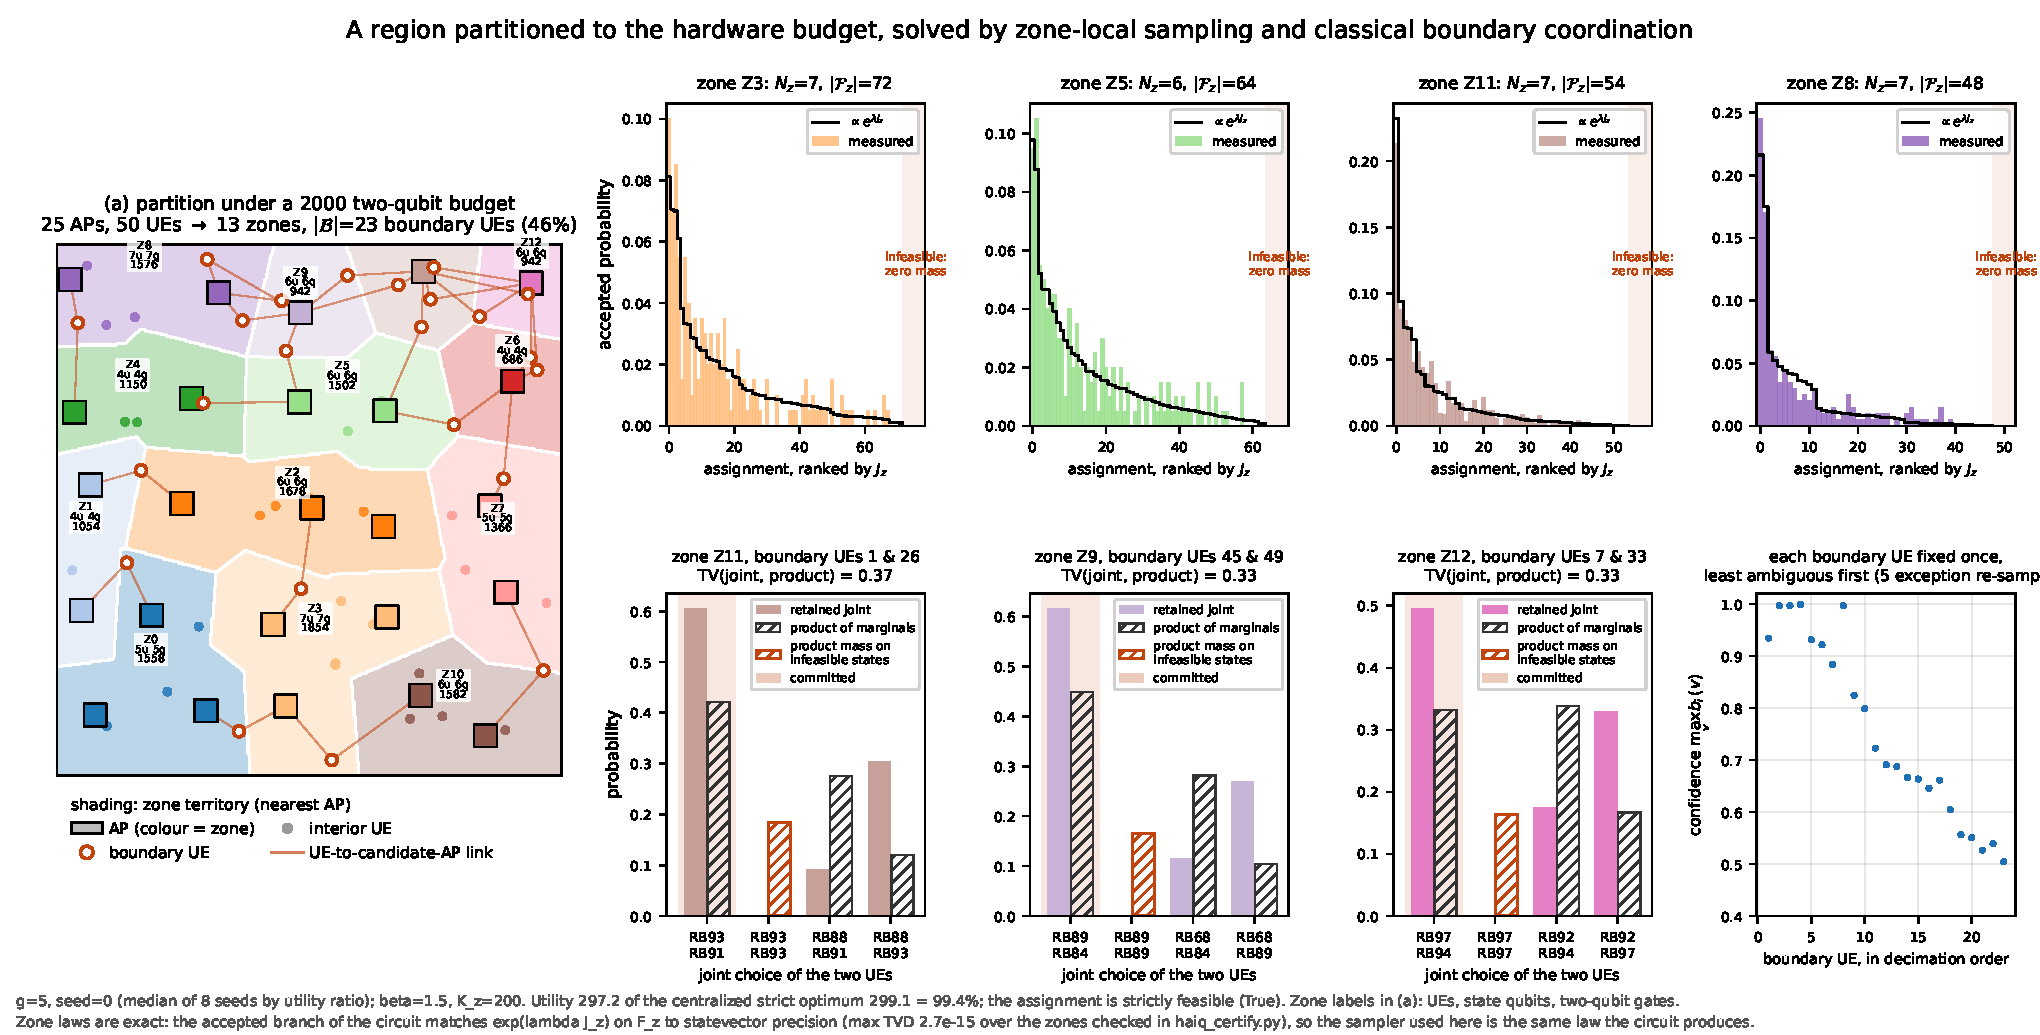
\includegraphics[width=\textwidth]{fig/fig_snapshot}
    \caption{Zone-local sampling and boundary coordination.}
    \label{fig:snapshot}
\end{figure*}

\subsection{One partitioned region}
\label{subsec:eval_snapshot}

Fig.~\ref{fig:snapshot} follows one campus instance of $M=25$ APs and $N=50$ UEs. It is drawn from a family of 16 seeds on the same map, 13 of which are globally feasible and supply the peer spread quoted below; the ablation of Fig.~\ref{fig:snapshot}(c3) uses a separate family of 16 instances spanning $g=4$ to $g=7$, of which 14 are feasible. Throughout, $J^{\star}$ is the centralized strict optimum from HiGHS. The partition gives $|\mathcal{Z}|=14$ zones within budget and $|\mathcal{B}|=23$ boundary UEs, so $46\%$ of the UEs require coordination, and the four displayed zone distributions match their exact accepted laws to $0.184$ at $K_z=200$ draws, with no mass outside $\mathcal{F}_z$ despite differing $\beta_z$.

On the two most dependent boundary-UE pairs the product of the marginals places $19\%$ of its belief on joint choices that violate a capacity condition the zone owns and that no sample in $\mathcal{S}_z$ realizes. Against a one-pass baseline identical in sampling and commitment rule, re-conditioning wins on 11 of the 14 ablation instances by $0.9$ percentage points of $J^{\star}$. Five re-samples add $62\%$ to the region's execution count. The result satisfies every capacity and consistency condition and reaches $98.7\%$ of $J^{\star}$, inside the $97.3$--$100.0\%$ spread of its peers, whose mean is $99.2\%$.

\begin{figure}[!t]
    \centering
    \includegraphics[width=\columnwidth]{fig/fig8}
    \caption{Zone-local computational cost.}
    \label{fig:zone_crossover}
\end{figure}

\subsection{What one zone circuit costs}
\label{subsec:eval_local_scaling}

For zone $z$, let $D_z=\sum_{i\in\mathcal{U}_z}|\mathcal{C}_i|$ denote the number of evaluated candidate edges, $\ell_{\max,z}=\max_{i\in\mathcal{U}_z}\lceil\log_2|\mathcal{C}_i|\rceil$ the widest candidate code, $Q_z^{\mathrm{cnt}}$ the counter width of \eqref{eq:counter-width}, and $\mathcal{M}_z$ the capacity conditions the zone owns, one per AP and RB it holds. With approximate-QFT arithmetic and standard multi-control decompositions, the modeled depth $T_z$ and two-qubit count $G_z$ of one oracle $\mathcal{O}_z$ scale as
\begin{equation}
    T_z,\;G_z=O\!\left(
    D_z\left(\ell_{\max,z}+Q_z^{\mathrm{cnt}}\right)
    +|\mathcal{M}_z|\,Q_z^{\mathrm{cnt}}
    \right).
    \label{eq:zone_one_pass_cost}
\end{equation}
Under bounded candidate degree and fixed counter width, both terms grow linearly with the zone size. Extra counters parallelize only the accumulation term, so adding counters has a floor.

Fig.~\ref{fig:zone_crossover} sets $D_z=2N_z$, $Q_z^{\mathrm{cnt}}=3$, and $|\mathcal{M}_z|=N_z$ for all quantum curves. Depths convert to logical latency as $\tau_z=T_z t_{\mathrm{layer}}$ with $t_{\mathrm{layer}}=12.5$~ns, and the enhanced schedule uses $R_{\mathrm{cnt}}=4$ parallel counters. Each method is charged one local pass, excluding repeated search rounds, accepted-draw repetitions, readout, queueing, and boundary coordination.

The classical reference is $\rho N_z^3$~ns with $\rho=0.400$, inside the $0.058$--$0.740$ range measured for the Hungarian method in~\cite{jang2025cqf}. It favors the classical side because that method omits the capacity constraints evaluated here. Crossovers occur at $N_z=17.7$ for the enhanced schedule, $31.1$ for the serial schedule, $36.5$ for GAS, and $42.1$ for QTG. The current partition produces zones of $1$--$13$ UEs, the largest measured circuit costing $1\,906$ gates; the fitted $G_z$ curve reaches $N_z\approx18$ at about $3\,500$ gates, or $76\%$ above the current $2000$-gate budget.

\begin{figure}[!t]
    \centering
    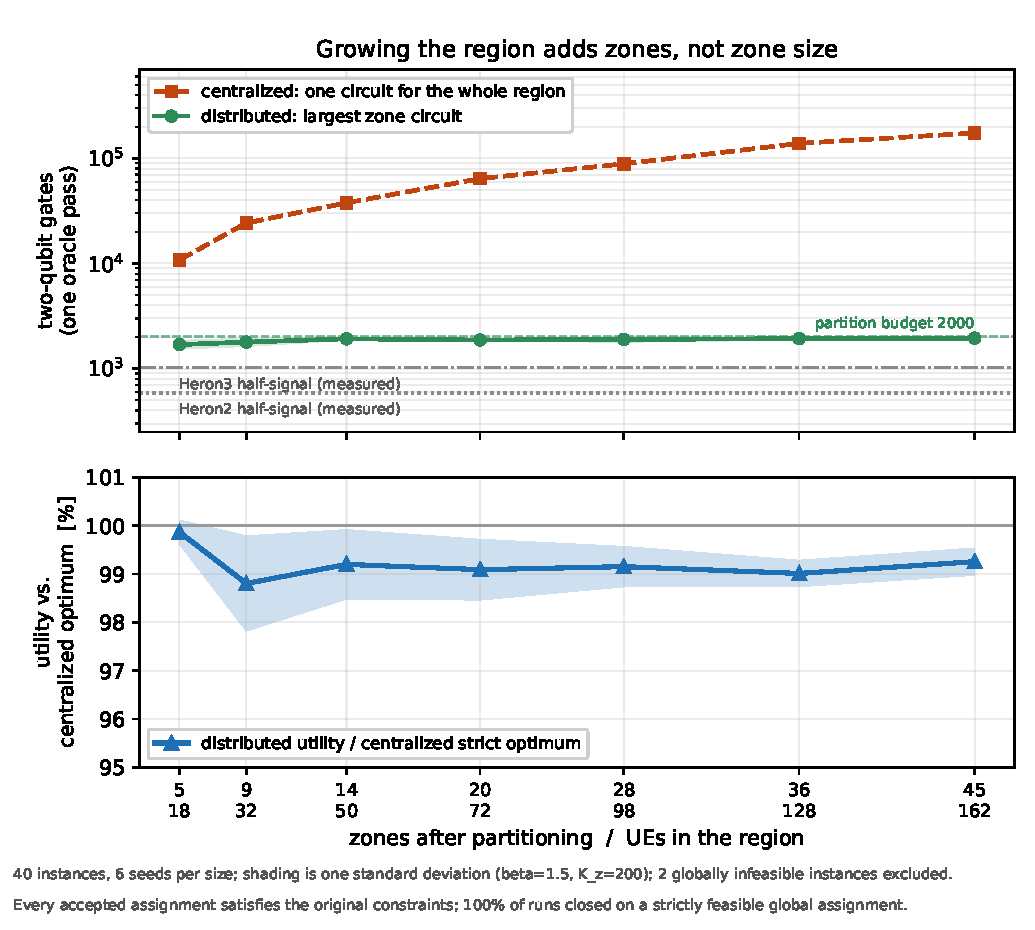
\includegraphics[width=\columnwidth]{fig/fig_scaling}
    \caption{Region-scale performance.}
    \label{fig:region_scaling}
\end{figure}

\subsection{What happens as the region grows}
\label{subsec:eval_network}

The region side is varied over $g=3,\ldots,9$ with six seeds per size; two of the 42 instances are globally infeasible and dropped, and the remaining 40 span $N=18$ to $N=162$ UEs and $|\mathcal{Z}|=5.3$ to $45.0$ zones on average, so the network grows ninefold at fixed local density. A centralized circuit for the whole region grows from $10\,801$ to $173\,983$ two-qubit gates, a factor of 16, while the largest zone circuit grows from $1\,693$ to $1\,950$, a factor of $1.15$, never leaving the partition budget: the hardware requirement follows deployment density rather than region size.

For zone $z$ with $n_z^{\mathrm{re}}$ re-samples, coordination traffic is modeled as $(1+n_z^{\mathrm{re}})K_z\bigl(\sum_{i\in\mathcal{B}_z}\lceil\log_2|\mathcal{C}_i|\rceil+32\bigr)$ bits, where the 32-bit field carries $J_z$ for the reconstruction of Appendix~\ref{app:reweighting}; the plotted values are converted to kilobytes. Regional traffic grows by $9.0\times$ as the zone count grows by $8.4\times$, so the mean report per zone increases by only $6\%$ and the per-zone load remains nearly unchanged as the region expands.

Averaged over the seeds at each region size, coordinated utility stays between $98.76\%$ and $99.32\%$ of $J^{\star}$ with no downward trend, and spans $96.79$--$100\%$ over the individual runs; all 40 finish globally feasible, so \eqref{eq:factorization} holds. Decomposition, finite sampling, and commitment cost about one percentage point, which does not accumulate over the evaluated range.

The exponent backoff keeps sampling affordable. On a separate 16-instance comparison covering 281 zones, reporting at the target exponent with $k=1$ costs between $1.4\times10^3$ and $2.8\times10^7$ executions depending on how tightly the zone is constrained; capping each zone at $10^4$ cuts the peak single-zone requirement by a factor of about $2\,800$, while mean utility is unchanged at $99.19\%$ of $J^{\star}$ and the largest single-instance loss is $0.74$ percentage points. Reconstruction is unbiased, so the cap trades effective sample size for execution cost rather than systematic bias.
}

% =====================================================================
{\color{purple}
\section{Conclusion}
\label{sec:conclusion}

This paper establishes a unified quantum framework for scalable network management through common assignment modeling, direct constraint
evaluation, and distributed coordination. Diverse inter-cell and intra-cell management tasks are represented within the same assignment
structure while preserving their respective objectives and resource constraints. The quantum computation directly evaluates the original
constraints and represents real-valued utilities through utility-dependent measurement probabilities, avoiding penalty reformulation and objective quantization. Zone-based decomposition extends the framework to network-scale problems under limited NISQ resources, while coordination of feasible local quantum outputs constructs a consistent network-wide assignment. Qiskit-based simulations and quantum-processor experiments demonstrate feasible solution generation and the scalability of the proposed computation. These results establish a common quantum computational approach for heterogeneous network assignment problems under present-day quantum resource limitations.

% =====================================================================
\appendices

\section{Exponential Utility Weight and Rotation Realization}
\label{app:exponential}

\subsection{Uniqueness of the exponential weight}
The zone decomposition in \eqref{eq:local-utility} expresses the network-wide utility as a sum of local utilities. To preserve this additive structure when the corresponding quantum weights are combined multiplicatively across zones, their product should depend on the local utilities only through their sum.

Let $f:\mathbb{R}\rightarrow(0,\infty)$ be a continuous local weight function for $|\mathcal Z|\geq2$. Suppose that
\begin{align}
\prod_{z\in\mathcal Z}f(J_z)=F\!\Big(\sum_{z\in\mathcal Z}J_z\Big),
\label{eq:app-weight-composition}
\end{align}
where $F$ is strictly increasing. Consider two local utilities $J_1$ and $J_2$, with all other zone utilities set to zero. Their product
weight is $f(J_1)f(J_2)f(0)^{|\mathcal Z|-2}$. Assigning the same total utility $J_1+J_2$ to a single zone gives $f(J_1+J_2)f(0)^{|\mathcal Z|-1}$. Since both cases have the same total utility, \eqref{eq:app-weight-composition} gives
\begin{align}
\frac{f(J_1)f(J_2)}{f(0)}=f(J_1+J_2).
\label{eq:app-cauchy}
\end{align}
Define the normalized weight as $\widetilde f(J)=f(J)/f(0)$. Then, \eqref{eq:app-cauchy} is expressed as
\begin{align}
\widetilde f(J_1)\widetilde f(J_2)=\widetilde f(J_1+J_2).
\label{eq:app-cauchy-normalized}
\end{align}
The continuous positive solutions of this exponential Cauchy equation have the form $\widetilde f(J)=e^{\lambda J}$ for a real constant $\lambda$, and the corresponding local weight is
\begin{align}
f(J)=f(0)e^{\lambda J},
\label{eq:app-exp-weight}
\end{align}
and the strict increase of $F$ gives $\lambda>0$. The exponential form is the unique continuous positive multiplicative weight, up to an assignment-independent factor, that preserves the additive utility relation under the zone decomposition.

\vspace{-3mm}
\subsection{Realization by controlled rotations}
The exponential weight is realized through the utility-qubit rotations defined in \eqref{eq:utility-angle}. For a complete local assignment $\bm z_z$, the assignment qubits specify the selected candidates, and the corresponding controlled rotations determine the probabilities of the utility qubits. According to \eqref{eq:utility-state}, selecting candidate $j$ for UE $i$ gives probability $g_{i,j}$ of observing its utility qubit in $\ket{0}$. The probability that all utility qubits satisfy this condition gives the zone-level utility weight $g_z(\bm z_z)$ defined in \eqref{eq:zone-utility-weight}.
Using the exponential mapping in \eqref{eq:utility-weight}, the zone-level weight can be expressed as
\begin{align}
g_z(\bm z_z)=\kappa_z\exp\!\left[\lambda J_z(\bm z_z)\right],
\label{eq:app-local-exponential}
\end{align}
where $\kappa_z>0$ is independent of the selected local assignment. The assignment-independent factor disappears when the probabilities
over feasible assignments are normalized. The resulting conditional distribution becomes \eqref{eq:conditional-exponential}. 
Also, zone-level weights preserve the network-wide utility under the decomposition. From \eqref{eq:local-utility},
\begin{align}
\prod_{z\in\mathcal Z}
g_z(\bm z_z)
\propto\exp\!\Big[\lambda\sum_{z\in\mathcal Z}J_z(\bm z_z)\Big]=\exp\!\left[\lambda J(\bm z)\right].
\label{eq:app-global-exponential}
\end{align}
The controlled rotations realize the multiplicative
exponential weighting established above while preserving the original
network-wide utility represented by the zone decomposition.

\vspace{-3mm}
\section{Coordination of Zone-Local Assignments}
\label{app:coordination}

%\vspace{-3mm}
\subsection{Reduction to boundary assignments}
\label{app:boundary-reduction}

Let $\mathcal B_z\subseteq\mathcal U_z$ denote the boundary UEs represented in zone $z$. For a local assignment $\bm z_z$, $\bm z_{\mathcal B_z}$ denotes its restriction to these boundary UEs, while the assignments of the remaining UEs are internal to the zone. Network-wide coordination concerns only the boundary assignments since the internal assignments do not appear in the consistency conditions between zones.
From \eqref{eq:factorization}, \eqref{eq:local-utility}, and \eqref{eq:composability}, the zone-local distributions in
\eqref{eq:conditional-exponential} recover the network-wide distribution when the boundary assignments are consistent across zones as
\begin{align}
p(\bm z)
\propto
\prod_{z\in\mathcal Z}p_z(\bm z_z)
\prod_{i\in\mathcal B}\delta_i(\bm z_i),
\label{eq:app-zone-law}
\end{align}
where $\delta_i(\bm z_i)$ is the consistency indicator in \eqref{eq:boundary-consistency}. For a boundary assignment $\bm s$,
the probability mass of the feasible local assignments consistent with $\bm s$ is
\begin{align}
p_z^{\mathrm b}(\bm s)=\sum_{\bm z_z\in\left\{\bm x\in\mathcal F_z:\bm x_{\mathcal B_z}=\bm s\right\}}p_z(\bm z_z).
\label{eq:app-boundary-factor}
\end{align}
Marginalizing \eqref{eq:app-zone-law} over the internal assignments gives
\begin{align}
p_{\mathcal B}(\bm z_{\mathcal B})\propto\prod_{z\in\mathcal Z}p_z^{\mathrm b}\!\left(\bm z_{\mathcal B_z}\right).
\label{eq:app-boundary-law}
\end{align}

\begin{proposition}[Boundary reduction]
\label{prop:app-boundary}
The reduction in \eqref{eq:app-boundary-factor} preserves the
network-wide distribution over the boundary assignments. Once the
boundary assignments are fixed consistently across zones, the internal
assignments can be determined independently within their respective
zones.
\end{proposition}

\begin{IEEEproof}
For a fixed consistent boundary assignment, all consistency indicators
$\delta_i$ equal one. The remaining factors in
\eqref{eq:app-zone-law} depend only on their respective zone-local
variables. Marginalizing each factor over its internal assignments
gives \eqref{eq:app-boundary-factor}, and their product gives
\eqref{eq:app-boundary-law}.
\end{IEEEproof}

Proposition~\ref{prop:app-boundary} reduces network-wide coordination
to the boundary assignments. Each zone estimates the joint boundary
distribution in \eqref{eq:app-boundary-factor} from its accepted
samples as
\begin{align}
\widehat p_z^{\mathrm b}(\bm s)
=
\frac{
\left|
\left\{
\bm z_z\in\mathcal S_z:
\bm z_{\mathcal B_z}=\bm s
\right\}
\right|
}{
|\mathcal S_z|
}.
\label{eq:app-empirical-boundary}
\end{align}
The resulting distribution preserves the relationship among boundary assignments represented by the joint local samples. The UE-wise marginals used for confidence-ordered coordination are obtained from these same samples as in \eqref{eq:boundary-marginal}.

\vspace{-3mm}
\subsection{Reweighting of zone-local samples}
\label{app:reweighting}

The sampling exponent can differ across zones according to their local quantum configurations. Let $\lambda_z\leq\lambda$ denote the exponent
used for sampling in zone $z$, where $\lambda$ is the common exponent used for coordination. Let $\bm z_z^{(n)}$ denote the $n$-th accepted
sample in that zone. Under local sampling, its relative probability is proportional to $\exp[\lambda_z J_z(\bm z_z^{(n)})]$, whereas the common exponent assigns a relative weight proportional to $\exp[\lambda J_z(\bm z_z^{(n)})]$. Their ratio gives the reweighting factor as
\begin{align}
w_z^{(n)}=\frac{\exp[\lambda J_z(\bm z_z^{(n)})]}{\exp[\lambda_z J_z(\bm z_z^{(n)})]}=\exp\!\left[(\lambda-\lambda_z)J_z(\bm z_z^{(n)})\right].
\label{eq:app-reweight}
\end{align}
Feasibility is evaluated independently of sampling exponent, and the feasible set $\mathcal F_z$ is unchanged. The weights in \eqref{eq:app-reweight} adjust the empirical local distribution from the sampling exponent $\lambda_z$ to the common coordination exponent $\lambda$.
A larger difference between $\lambda$ and $\lambda_z$ can concentrate the reweighted probability mass on a smaller number of accepted samples. This concentration is measured by the effective sample size
\begin{align}
\widetilde K_z=\frac{(\sum_{n=1}^{K_z}w_z^{(n)})^2}{\sum_{n=1}^{K_z}(w_z^{(n)})^2},
\label{eq:app-ess}
\end{align}
where $K_z=|\mathcal S_z|$. The effective sample size equals $K_z$ when the sample weights are uniform and approaches one when a single sample dominates the total weight. Since $\widetilde K_z\leq K_z$, $\widetilde K_z$ provides the sample sufficiency measure used during coordination.
The reweighting factors in \eqref{eq:app-reweight} give the sample weights in the empirical marginal \eqref{eq:boundary-marginal}. The joint boundary distribution $\widehat p_z^{\mathrm b}$ in \eqref{eq:app-empirical-boundary} is reweighted in the same manner by summing the weights of the samples associated with each boundary assignment. When $\lambda_z=\lambda$, all $w_z^{(n)}=1$, and weighted estimates reduce to their unweighted empirical forms.

\vspace{-3mm}
\subsection{Confidence-ordered decimation}
\label{app:decimation}

Confidence-ordered decimation resolves the boundary assignments one UE at a time while preserving the assignment relationships contained in
the joint local samples. At the $t$-th iteration, let $\mathcal S_z^{(t)}$ denote the current sample set in zone $z$, and let
$\pi_{z,i}^{(t)}(j)$ denote the corresponding marginal probability for an unresolved boundary UE $i$. The marginals from zones containing
UE $i$ obtain the consensus distribution as
\begin{align}
b_i^{(t)}(j)=\frac{\prod_{z\in\mathcal Z_i}\pi_{z,i}^{(t)}(j)}{\sum_{j'\in\mathcal C_i}\prod_{z\in\mathcal Z_i}\pi_{z,i}^{(t)}(j')}.
\label{eq:app-consensus}
\end{align}
The concentration of this distribution is measured using the normalized
entropy defined as
\begin{align}
\gamma_i^{(t)}
=1+\frac{\sum_{j\in\mathcal C_i}b_i^{(t)}(j)\log b_i^{(t)}(j)}{\log|\mathcal C_i|}.
\label{eq:app-confidence}
\end{align}
A larger $\gamma_i^{(t)}$ indicates a stronger preference for a
particular candidate. Note that a uniform consensus gives
$\gamma_i^{(t)}=0$.
Among the unresolved boundary UEs, the UE with the largest confidence
is selected as
\begin{align}
i^\star=\arg\max_{i\in\mathcal B_{\mathrm u}^{(t)}}\gamma_i^{(t)},
\label{eq:app-select-ue}
\end{align}
where $\mathcal B_{\mathrm u}^{(t)}$ denotes the set of unresolved
boundary UEs at the $t$-th iteration. The candidate with the largest consensus
probability for the selected UE is
\begin{align}
j^\star=\arg\max_{j\in\mathcal C_{i^\star}}b_{i^\star}^{(t)}(j).
\label{eq:app-select-candidate}
\end{align}
UE $i^\star$ is fixed to candidate $j^\star$. For each zone containing
this UE, the joint sample set is filtered according to
\begin{align}
\mathcal S_z^{(t+1)}
=
\left\{
\bm z_z\in\mathcal S_z^{(t)}:
z_{i^\star,j^\star}=1
\right\}.
\label{eq:app-filter}
\end{align}
The sample sets of the other zones remain unchanged.

Since each sample specifies a complete local assignment, filtering one boundary UE also changes empirical candidate distributions of
unresolved boundary UEs in the affected zones. Their marginal, consensus, and confidence values are recomputed from the filtered sample sets before the next boundary UE is selected. Applying the filtering operation to the joint samples, rather than directly modifying their marginals, preserves the assignment relationships represented by local quantum outputs.
Filtering can reduce the effective sample size $\widetilde K_z$. If $\widetilde K_z<K_{\min}$ in an affected zone, that zone is sampled again with its already resolved boundary assignments fixed during state preparation. Only the affected zone is sampled again, and he sample sets of the other zones remain unchanged. In practrice, a small pseudo-count can be added when estimating empirical marginals to prevent a candidate that is absent from a finite sample set from producing a zero consensus probability.
The procedure terminates after at most $|\mathcal B|$ decimation steps, when all boundary UEs have consistent assignments across their
corresponding zones. The remaining local samples satisfy their zone-level feasibility conditions, and the resolved boundary assignments satisfy the consistency conditions in \eqref{eq:factorization}. Algorithm~\ref{alg:decimation} summarizes the overall procedure.

\begin{algorithm}[!t]
\caption{Confidence-ordered decimation}
\label{alg:decimation}
\begin{algorithmic}[1]
\STATE $t\leftarrow0$
\STATE $\mathcal S_z^{(0)}\leftarrow\mathcal S_z$ for all
$z\in\mathcal Z$
\STATE $\mathcal B_{\mathrm u}^{(0)}\leftarrow\mathcal B$
\WHILE{$\mathcal B_{\mathrm u}^{(t)}\neq\varnothing$}
\STATE compute $\pi_{z,i}^{(t)}$ from the current weighted samples
\STATE compute $b_i^{(t)}$ by \eqref{eq:app-consensus}
\STATE compute $\gamma_i^{(t)}$ by \eqref{eq:app-confidence}
\STATE select $i^\star$ by \eqref{eq:app-select-ue}
\STATE select $j^\star$ by \eqref{eq:app-select-candidate}
\STATE fix UE $i^\star$ to candidate $j^\star$
\STATE filter the affected sample sets by \eqref{eq:app-filter}
\IF{$\widetilde K_z<K_{\min}$ for an affected zone $z$}
\STATE re-sample zone $z$ with its resolved boundary assignments fixed
\ENDIF
\STATE $\mathcal B_{\mathrm u}^{(t+1)}
\leftarrow
\mathcal B_{\mathrm u}^{(t)}\setminus\{i^\star\}$
\STATE $t\leftarrow t+1$
\ENDWHILE
\end{algorithmic}
\end{algorithm}

}

% =====================================================================
%\section*{Acknowledgment}
% This work was supported by the National Research Foundation of
% Korea (NRF) grant funded by the Korea government (MSIT)
% (2022R1A5A1027646 and RS-2025-00563388).
% =====================================================================
\begin{thebibliography}{60}

% -- prior version (delta anchor) --
\bibitem{jang2025cqf}
Y. H. Jang, J. Hwang, W. Lee, H. S. Kim, and S. H. Lee, ``A unified
quantum framework for assignment optimization in network
administration,'' \emph{IEEE Commun. Mag.}, 2025.
% FIXME(submission): insert final volume, issue, pages, and DOI from
% the published IEEE record.

% -- network administration context --
\bibitem{lee2024node}
S. H. Lee \emph{et al.}, ``A node-cooperative universal framework
for wireless network management automation,'' \emph{IEEE Commun.
Mag.}, vol. 62, no. 6, pp. 50-57, Jun. 2024.

\bibitem{masaracchia2023dt}
A. Masaracchia, V. Sharma, M. Fahim, O. A. Dobre, and T. Q. Duong,
``Digital twin for open RAN: Toward intelligent and resilient 6G
radio access networks,'' \emph{IEEE Commun. Mag.}, vol. 61, no. 11,
pp. 112-118, Nov. 2023.

\bibitem{wang2022quantum6g}
C. Wang and A. Rahman, ``Quantum-enabled 6G wireless networks:
Opportunities and challenges,'' \emph{IEEE Wireless Commun.},
vol. 29, no. 1, pp. 58-69, Feb. 2022.

\bibitem{yi2025towards}
W. Yi \emph{et al.}, ``Towards seamless 6G and AI/ML convergence:
Architectural enhancements and security challenges,'' \emph{IEEE
Netw.}, vol. 39, no. 4, pp. 157-165, 2025.

\bibitem{chowdhary2022intent}
A. Chowdhary, A. Sabur, N. Vadnere, and D. Huang, ``Intent-driven
security policy management for software-defined systems,''
\emph{IEEE Trans. Netw. Service Manag.}, vol. 19, no. 4,
pp. 5208-5223, Dec. 2022.

\bibitem{brassard2002}
G. Brassard, P. H\o yer, M. Mosca, and A. Tapp, ``Quantum amplitude
amplification and estimation,'' \emph{Contemp. Math.}, vol. 305,
pp. 53-74, 2002.

\bibitem{farhi2014}
E. Farhi, J. Goldstone, and S. Gutmann, ``A quantum approximate
optimization algorithm,'' arXiv:1411.4028, 2014.

\bibitem{lucas2014}
A. Lucas, ``Ising formulations of many NP problems,''
\emph{Front. Phys.}, vol. 2, p. 5, 2014.

\bibitem{botsinis2019}
P. Botsinis \emph{et al.}, ``Quantum search algorithms for wireless
communications,'' \emph{IEEE Commun. Surveys Tuts.}, vol. 21, no. 2,
pp. 1209-1242, 2nd Quart. 2019.

\bibitem{kadowaki1998}
T. Kadowaki and H. Nishimori, ``Quantum annealing in the transverse
Ising model,'' \emph{Phys. Rev. E}, vol. 58, no. 5, pp. 5355-5363,
Nov. 1998.

% -- quantum algorithm primary sources --
\bibitem{nielsen2011}
M. A. Nielsen and I. L. Chuang, \emph{Quantum Computation and
Quantum Information}. Cambridge, U.K.: Cambridge Univ. Press, 2011.

\bibitem{grover1996}
L. K. Grover, ``A fast quantum mechanical algorithm for database
search,'' in \emph{Proc. 28th ACM Symp. Theory Comput. (STOC)},
1996, pp. 212-219.

\bibitem{boyer1998}
M. Boyer, G. Brassard, P. H\o yer, and A. Tapp, ``Tight bounds on
quantum searching,'' \emph{Fortschr. Phys.}, vol. 46, no. 4-5,
pp. 493-505, 1998.

\bibitem{durr1996}
C. D\"urr and P. H\o yer, ``A quantum algorithm for finding the
minimum,'' arXiv:quant-ph/9607014, 1996.

\bibitem{biamonte2017}
J. Biamonte \emph{et al.}, ``Quantum machine learning,''
\emph{Nature}, vol. 549, no. 7671, pp. 195-202, 2017.

\bibitem{ngoenriang2023}
N. Ngoenriang \emph{et al.}, ``DQC\textsuperscript{2}O: Distributed
quantum computing for collaborative optimization in future
networks,'' \emph{IEEE Commun. Mag.}, vol. 61, no. 5, pp. 188-194,
May 2023.

\bibitem{kim2021heuristic}
M. Kim \emph{et al.}, ``Heuristic quantum optimization for 6G
wireless communications,'' \emph{IEEE Netw.}, vol. 35, no. 4,
pp. 8-15, Jul./Aug. 2021.

\bibitem{seo2022}
Y. Seo, Y. Kang, and J. Heo, ``Quantum search algorithm for
weighted solutions,'' \emph{IEEE Access}, vol. 10,
pp. 16209-16224, 2022.

\bibitem{fan2022hybrid}
L. Fan \emph{et al.}, ``Hybrid quantum-classical computing for
future network optimization,'' \emph{IEEE Netw.}, vol. 36, no. 5,
pp. 72-76, Sep./Oct. 2022.

% -- oracle-based search over constrained binary domains --
\bibitem{gilliam2021gas}
A. Gilliam, S. Woerner, and C. Gonciulea, ``Grover adaptive search
for constrained polynomial binary optimization,'' \emph{Quantum},
vol. 5, p. 428, Apr. 2021.

\bibitem{fujiwara2025gas}
S. Fujiwara and N. Ishikawa, ``Grover adaptive search with spin
variables,'' \emph{IEEE Trans. Quantum Eng.}, 2025,
doi: 10.1109/TQE.2025.3595910.
% FIXME(submission): confirm final volume and article number.

\bibitem{wilkening2025qtg}
S. Wilkening, A.-I. Lefterovici, L. Binkowski, M. Perk, S. P.
Fekete, and T. J. Osborne, ``A quantum algorithm for solving 0-1
knapsack problems,'' \emph{npj Quantum Inf.}, vol. 11, art. no.
146, Aug. 2025.

\bibitem{wilkening2025qkp}
S. Wilkening \emph{et al.}, ``A quantum search method for quadratic
and multidimensional knapsack problems,'' arXiv:2503.22325, 2025.
% FIXME(submission): check for a journal version.

% -- quantum optimization for network management --
\bibitem{narottama2022qnn}
B. Narottama and S. Y. Shin, ``Quantum neural networks for resource
allocation in wireless communications,'' \emph{IEEE Trans. Wireless
Commun.}, vol. 21, no. 2, pp. 1103-1116, Feb. 2022.

\bibitem{ansere2024qdrl}
J. A. Ansere, E. Gyamfi, V. Sharma, H. Shin, O. A. Dobre, and
T. Q. Duong, ``Quantum deep reinforcement learning for dynamic
resource allocation in mobile edge computing-based IoT systems,''
\emph{IEEE Trans. Wireless Commun.}, vol. 23, no. 6,
pp. 6221-6233, Jun. 2024.

\bibitem{ansere2026tnse}
J. A. Ansere, S. C. Prabhashana, N. Simmons, O. A. Dobre, H. Shin,
and T. Q. Duong, ``Quantum deep deterministic policy gradient for
digital twin-enabled semantic IoV networks,'' \emph{IEEE Trans.
Netw. Sci. Eng.}, vol. 13, pp. 54-66, 2026.

\bibitem{zhang2024tnse}
Y. Zhang, Y. Gong, L. Fan, Y. Wang, Z. Han, and Y. Guo,
``Quantum-assisted joint caching and power allocation for
integrated satellite-terrestrial networks,'' \emph{IEEE Trans.
Netw. Sci. Eng.}, vol. 11, no. 6, pp. 5163-5174, Nov./Dec. 2024.

\bibitem{wei2024tnse}
X. Wei, L. Fan, Y. Guo, Y. Gong, Z. Han, and Y. Wang, ``Hybrid
quantum-classical Benders' decomposition for federated learning
scheduling in distributed networks,'' \emph{IEEE Trans. Netw. Sci.
Eng.}, vol. 11, no. 6, pp. 6038-6051, Nov./Dec. 2024.

\bibitem{zhang2024beamforming}
J. Zhang, G. Zheng, T. Koike-Akino, K.-K. Wong, and F. A. Burton,
``Hybrid quantum-classical neural networks for downlink
beamforming optimization,'' \emph{IEEE Trans. Wireless Commun.},
vol. 23, no. 11, pp. 16498-16512, Nov. 2024.

\bibitem{sharma2026tnse}
A. Sharma, K. Singh, A. Paul, K. Agrawal, K. Dev, and S. Biswas,
``Quantum-driven resource optimization for full-duplex
STAR-RIS-aided NOMA-ISAC with constraint projection,''
\emph{IEEE Trans. Netw. Sci. Eng.}, vol. 13, pp. 6827-6842, 2026.

% -- circuit primitives (code-enforced citations) --
\bibitem{draper2000}
T. G. Draper, ``Addition on a quantum computer,''
arXiv:quant-ph/0008033, 2000.

\bibitem{coppersmith1994}
D. Coppersmith, ``An approximate Fourier transform useful in quantum
factoring,'' IBM Res. Rep. RC19642, 1994; arXiv:quant-ph/0201067.

\bibitem{maslov2016}
D. Maslov, ``Advantages of using relative-phase Toffoli gates with
an application to multiple control Toffoli optimization,''
\emph{Phys. Rev. A}, vol. 93, p. 022311, 2016.

\bibitem{campbell2019}
E. Campbell, A. Khurana, and A. Montanaro, ``Applying quantum
algorithms to constraint satisfaction problems,'' \emph{Quantum},
vol. 3, p. 167, 2019.

\bibitem{preskill2018}
J. Preskill, ``Quantum computing in the NISQ era and beyond,''
\emph{Quantum}, vol. 2, p. 79, 2018.

\bibitem{qiskit}
Qiskit contributors, ``Qiskit: An open-source framework for quantum
computing,'' 2023. [Online]. Available: \url{https://qiskit.org}

% -- classical baselines & models --
\bibitem{kuhn1955}
H. W. Kuhn, ``The Hungarian method for the assignment problem,''
\emph{Nav. Res. Logist. Q.}, vol. 2, pp. 83-97, 1955.

\bibitem{tr36873}
3GPP, ``Study on 3D channel model for LTE,'' TR 36.873, 2017.

% REMOVED in rev.2: li2017temporal (Li et al., Science, 2017).
% It was the sole support for "per-cell density remains bounded even
% as the global network grows" in Sec. VII, i.e. for q_local = O(1)
% in N. That paper concerns controllability of temporal networks and
% does not establish the claim. The claim is now stated as a
% deployment assumption. Reinstate only with a reference that
% actually bounds cellular user density.

% -- artifact --
\bibitem{cqfrepo}
``CQF public repository,'' GitHub. [Online]. Available:
\url{https://github.com/gyh1238/CQF}

% -- rev.2 status: 40 references (was 29).
%  Still open toward the 55-65 target of checklist item 12:
%  dynamic-decoupling and readout-mitigation primary sources
%  (currently claimed in Sec. VI-A with no citation), an integer
%  comparator reference distinct from the Qiskit manual, a
%  cellular deployment-density reference (see li2017temporal note
%  above), and per-row citations should Table I gain an
%  annealing-hardware or QAOA-network-application row.

\end{thebibliography}

\vskip -2\baselineskip plus -1fil

\begin{IEEEbiographynophoto}
%[{\includegraphics[width=1in,height=1.25in,clip,keepaspectratio]{fig/jang_yonghun.jpg}}]
{Yong Hun Jang} %(disclose@korea.ac.kr)
received the B.S. degree from the Seoul National University of Science and Technology in 2019. He is currently with the School of Electrical Engineering, Korea University, Seoul, South Korea. His research interests include distributed system optimization, computing cluster parallelization and job scheduling, intelligent reflecting surface for wireless communication and their applications.
\end{IEEEbiographynophoto}

\vskip -2\baselineskip plus -1fil

\begin{IEEEbiographynophoto}
{Sang Hyun Lee} %(sanghyunlee@korea.ac.kr)
received the B.S. and M.S. degrees from the Korea Advanced Institute of Science and Technology in 1999 and 2001, respectively, and the Ph.D. degree from the University of Texas at Austin in 2011. He is currently with the School of Electrical Engineering, Korea University, Seoul, Korea. His research interests include communications, designs, and optimizations on wireless applications in high-performance computing.
\end{IEEEbiographynophoto}

\end{document}

% Constrained Quantum Optimization at Utility Scale: Application to the Knapsack Problem

% Combinatorial Optimization Enhanced by Shallow Quantum Circuits with 104 Superconducting Qubits

% Scaling Whole-Chip QAOA for Higher-Order Ising Spin Glass Models on Heavy-Hex Graphs

% Quantum-Enhanced Greedy Combinatorial Optimization Solver

% Quantum Approximate Optimization of Non-Planar Graph Problems on a Planar Superconducting Processor
